\appendix
\onecolumn


\section{Implementation Details} \label{appendix:full_implementation_details}

\subsection{Scenario Generation} \label{appendix:scenario_generation}

We adopt a Self-Instruct style expansion~\citep{selfinstruct} to scale from 100 seed websites to 1,000 diverse scenarios.
The seed set is drawn from popular domain names\footnote{\url{https://www.similarweb.com/top-websites/}}, and the LLM generates new candidates conditioned on few-shot examples that emphasize stateful, database-backed interactions.
To maintain diversity, we apply two complementary filters: (1) an LLM classifier that scores each candidate on suitability for CRUD operations (create, read, update, delete), rejecting content-centric or read-only scenarios (e.g., news), and (2) embedding-based deduplication using cosine similarity with a threshold of 0.85, ensuring newly generated scenarios are sufficiently distinct from the existing pool.
We also enforce category caps to prevent over-representation of dominant types such as e-commerce.
The prompts used for generation and classification are provided in Figures~\ref{fig:gen-scenario-system} and \ref{fig:gen-scenario-user}.
Table~\ref{tab:scenarios_demo} shows a random sample of 100 generated scenarios.
We also show the distribution of the synthesized scenarios in Figure~\ref{fig:domain_distribution} and the wordcloud of the scenario descriptions in Figure~\ref{fig:wordcloud}.
The distribution shows that the synthesized scenarios span diverse domains without collapsing to a few dominant types.

\subsection{Task Generation} \label{appendix:task_generation}

For each scenario, we prompt the LLM to generate $k=10$ diverse user tasks that serve as functional requirements for downstream synthesis.
This modest count keeps the database schema and toolset implementation tractable for LLMs.
The prompt enforces two constraints: (1) tasks must be API-solvable without UI dependencies such as clicking or page navigation, and (2) tasks assume post-authentication context to unlock deeper functionalities.
Each task is required to be specific and self-contained, including concrete parameters (e.g., product IDs, user names) so that it can be executed without additional clarification.
This requirement-driven design ensures that the subsequently generated database schema and toolset are aligned with actual user needs rather than being over-specified or incomplete.
The prompt template is shown in Figure~\ref{fig:gen-task}. And the generated tasks are shown in Table~\ref{tab:tasks_demo}.

\subsection{Environment Synthesis} \label{appendix:environment_synthesis}

This section details the synthesis of the three core POMDP components: state space (database), action and observation spaces (interface), and reward function (verification).

\myparagraph{Database Schema Generation.}
Given the scenario description and task set $\mathcal{T}_{E_i}$, the LLM infers the minimal relational schema required to make all tasks feasible.
The output is a set of SQLite DDL statements defining tables, columns, types, primary keys, foreign keys, and indexes.
We instruct the LLM to reason about entity relationships implied by the tasks (e.g., a ``cancel order'' task implies an Orders table with a status column) and to avoid authentication-related fields.
Based on the introduced self-correction mechanism, we attempt to run the generated DDL statements in an isolated environment and test the functionality.
If any DDL statement fails execution, we capture the error message, summarize it via a separate LLM call, and append the summary to the prompt for regeneration.
This feedback loop repeats with an error threshold of 10\%: if fewer than 10\% of tables fail, we accept the schema.
The prompt is shown in Figure~\ref{fig:gen-db}. And we visualize part of the SQLite database schema with sample data in Figure~\ref{fig:database_view}.

\myparagraph{Sample Data Synthesis.}
An empty schema is insufficient for task execution, since many tasks require querying or updating existing records.
We synthesize sample data by prompting the LLM to analyze task preconditions and generate INSERT statements that satisfy them.
For example, if a task requires ``updating product inventory,'' the synthesized data must include at least one product with a non-zero stock level.
The LLM outputs a JSON structure containing table names and corresponding INSERT statements, which are executed in dependency order respecting foreign key constraints.
We apply the same error-feedback loop as schema generation, with an error threshold of 10\% for acceptable insert failures.
The prompt is shown in Figures~\ref{fig:gen-data-1} and \ref{fig:gen-data-2}. 

\myparagraph{Interface Specification Design.}
Before generating implementation code, we first synthesize an interface specification that defines the toolset schema.
This two-stage approach (schema then code) reduces hallucination in long code generation, since pilot experiments show that direct code generation for environments with 30+ tools often produces inconsistent interfaces.
Given the task set and database schema, the LLM infers the minimal set of endpoints required to make every task executable.
Each endpoint specification includes: name, method, path, summary, typed input parameters, and response schema.
The specification also serves as documentation for agents at inference time, shown in Table~\ref{tab:demo_api_schema}.
The prompt is shown in Figures~\ref{fig:gen-api-1} and \ref{fig:gen-api-2}, and an example of the synthesized MCP toolset is shown in Figure~\ref{fig:toolset-demo}.

\myparagraph{Environment Implementation.}
With the API specification and database schema, we generate a complete Python file implementing an MCP server.
The generated code includes: SQLAlchemy ORM models mirroring the database schema, Pydantic request/response models, and FastAPI endpoint handlers that perform database operations.
Each environment averages about 2,000 lines of code and exposes 35 tools on average.
After generation, we validate the environment by launching and checking that the MCP server starts successfully and responds to health checks and ``list tools'' calls.
Failed environments enter the self-correction loop to fix the errors.
The prompt is shown in Figures~\ref{fig:gen-env-1}, \ref{fig:gen-env-2}, and \ref{fig:gen-env-3}.

\myparagraph{Verification Code Synthesis.}
For each task, we generate a Python verification function that compares database states before and after agent execution.
The function takes two database paths (initial and final) as input, executes SQL queries to extract task-relevant information, and returns a structured dictionary containing: changed records, expected outcomes, and diagnostic signals.
We also generate success and failure criteria in natural language that guide the LLM-as-a-Judge in interpreting the verification results.
During RL training, this code-augmented verification provides grounded evidence to the judge, reducing hallucination in reward assignment.
The prompt for generating the verification code is shown in Table~\ref{tab:verification-prompt-2}, and the example of the synthesized verification code is shown in Figure~\ref{fig:verification-code-part1} and~\ref{fig:verification-code-part2}.

\myparagraph{Self-Correction Mechanism.}
All synthesis stages share a common error-recovery pattern.
When generated code fails execution, we capture the full error traceback and invoke a separate LLM call to produce a concise error summary (typically 200-500 tokens) that identifies the root cause and suggests fixes.
This summary is appended to the original prompt for the next generation attempt.
We limit retries to 5 iterations per component.
If an error threshold (10\% for schema/data, 0\% for environment startup) is exceeded after all retries, we select the best attempt based on error rate and proceed.
This approach achieves over 85\% first-attempt success rate across all stages, with an average of 1.13 correction iterations for failed cases.


\subsection{Tool Calling Format and Validation} \label{appendix:tool_call_format}

We adopt the Qwen3 tool-calling format~\citep{qwen3}, which wraps each tool invocation in XML tags: ``\texttt{<tool\_call>}\{name: \dots, arguments: \dots\}\texttt{</tool\_call>}''.
Rather than exposing all environment-specific tools directly to the agent, we design a two-level abstraction that decouples the agent from environment details.

\myparagraph{Two-Level Tool Abstraction}
The agent interacts with MCP environments through exactly two meta-tools:
(1) \texttt{list\_tools}, which queries the MCP server to retrieve all available tools in the current environment along with their metadata (input/output schemas, descriptions), and
(2) \texttt{call\_tool}, which invokes an environment-specific tool by name with the required arguments passed as a JSON string.
This design enables the agent to dynamically discover and invoke different toolsets across environments without hardcoding any tool information.
The complete system prompt is shown in Figure~\ref{fig:agent-system-prompt}.

\myparagraph{Format Validation Rules}
During RL training, we enforce format constraints to ensure well-formed tool calls and prevent hallucinated or malformed interactions.
We apply rule-based validation at each step of the trajectory, classifying it as either valid, a format error, or an environment/server error.
The validation checks the following conditions:
(1) Reasoning format: All assistant messages must contain non-empty reasoning within \texttt{<think>...</think>} tags.
(2) Tool name validity: The agent must not call hallucinated tools (tools not returned by \texttt{list\_tools}) or use invalid tool names.
(3) Argument validity: Tool arguments must be well-formed JSON that conforms to the tool schema.
(4) Protocol adherence: The agent must call \texttt{list\_tools} exactly once, and it must be the first tool call in the trajectory.
(5) Interaction consistency: If the agent produces multiple interaction turns, it must make at least one successful tool call beyond the initial \texttt{list\_tools}.
(6) Server response: Each tool call must receive a non-error response from the MCP server. For example, if the server returns an error message indicating timeout or internal failure, we classify it as an environment error.
For each step $t$, if any of the 1-5 conditions are violated, we classify it as a format error, assigning a negative reward $r_t = -1$. If condition 6 is violated, we classify it as an environment error with reward $r_t = 0$ following the reward shapes in Sec.~\ref{sec:reward_design}. 

\myparagraph{Early Termination}
To improve training efficiency, we implement early stopping for unrecoverable errors.
When the validator detects a format error or server error during rollout, we terminate the trajectory immediately rather than continuing to generate additional steps.
This saves computational resources and prevents the agent from receiving reward signals for fundamentally broken trajectories. 


\subsection{Training and Evaluation Details} \label{appendix:implementation_details}

\myparagraph{Training Hyperparameters.}
Table~\ref{tab:rl_hyper} summarizes the hyperparameters used for GRPO training~\citep{shao2024deepseekmath}.
According to the common agentic RL training settings~\citep{li2025simulatingenvironmentsreasoningmodels,wang2025ragenunderstandingselfevolutionllm}, we set the KL coefficient to 0.001.
Beyond standard GRPO settings, we use a higher clip ratio of 0.28, following the recommendation in DAPO~\citep{dapo} to allow more exploration for the agent.
Also, we use sequence-level importance sampling to mitigate the distribution shift issue between the rollout engine and the model training engine~\citep{yao2025offpolicy}.

\myparagraph{Environment Management.}
We implement multi-turn RL training on top of AgentFly~\citep{wang2025agentfly} and verl~\citep{verl}.
Each training step launches 1,024 isolated environment instances in parallel, with each instance running as an independent MCP server backed by its own SQLite database copy.
This isolation ensures that concurrent rollouts do not interfere with each other's state transitions.
Environment instances are reset by restoring the database to its initial state after each rollout completes.
Environment startup (spawning MCP servers, copying databases) is a bottleneck in online RL, as it blocks rollout collection.
To overlap environment preparation with policy training, we further implement a pre-fetching mechanism: while the current batch undergoes gradient updates, a background thread pre-configures environments for the next batch.
This significantly reduces per-step wall-clock time compared to sequential environment startup.

\myparagraph{Sample Splitting for History-Aware Training.}
As described in Section~\ref{sec:history_aware_training}, we align training with inference by applying history truncation during optimization.
We use simple history context management, specifically sliding window truncation, to study the mismatch issue between training and inference.
Specifically, given a completed rollout with $T$ assistant turns, we split it into $T$ separate training samples.
For sample $t$, the input consists of the system prompt, initial user message, the first assistant-tool exchange (which contains the \texttt{list\_tools} call), and the $w=3$ most recent turns preceding turn $t$.
The loss is computed only on the tokens of turn $t$, while all preceding context tokens have their loss mask set to zero.
This ``sample splitting'' approach ensures each training sample mirrors the truncated context the agent will see at inference time. Although this increases the number of forward passes per rollout by a factor of $T$, it eliminates the distribution shift that would otherwise occur when training on full histories but deploying with truncated contexts.
More complex history context management is possible, but it is beyond the scope of this paper.

\myparagraph{Reward Computation.}
At the end of each rollout, we invoke the code-augmented LLM-as-a-Judge to determine task completion status.
The verification code is executed on the final database state, comparing it against the initial state, and its structured output (changed records, success criteria) is provided to GPT-5~\citep{openai_gpt5_2025} along with the agent trajectory.
The judge returns one of four classifications: \texttt{Completed}, \texttt{Partially Completed}, \texttt{Agent Error}, or \texttt{Environment Error}.
We map these to rewards as specified in Sec.~\ref{sec:reward_design}.
To reduce latency, verification calls are batched and executed asynchronously while the next rollout batch is being collected, adding negligible overhead to the training loop.

\myparagraph{Evaluation Protocol.}
We evaluate trained agents on three benchmarks that differ substantially from our training distribution.
A key challenge is that each benchmark uses a different tool-calling format: \taubench~\citep{taubench2,verified_tau2} expects direct tool names (e.g., \texttt{get\_user\_details}), BFCLv3~\citep{bfcl} uses function-calling syntax, and MCP-Universe~\citep{mcpuniverse} uses the MCP protocol.
To bridge this gap, we implement format converters that translate between our unified \texttt{call\_tool} abstraction and each benchmark's native format.
For \taubench, we wrap each tool call as \texttt{call\_tool(tool\_name="mcp\_tool\_\{name\}", arguments=\{...\})} and unwrap responses accordingly.
For BFCLv3, we aggregate multi-turn trajectories into the expected single-turn or parallel function call format, skipping \texttt{list\_tools} meta-calls.
This ensures evaluation measures the agent's actual task-solving ability rather than format compliance.

\myparagraph{Decoding and Context Configuration.}
During evaluation, we use temperature 0.6 with top-$k$=20 and top-$p$=0.95, following the recommended decoding settings in Qwen3~\citep{qwen3}.
We extend the context window to 131,072 tokens via RoPE scaling~\citep{rope} for all evaluations, as some benchmark tasks (especially BFCLv3 multi-turn categories) require processing lengthy interaction histories.
When processing long context tasks, the history limit is loosened to $w=10$ turns during evaluation, allowing agents to leverage more context information.

\begin{table}[t]
\centering
\caption{Hyperparameters for GRPO training.}
\label{tab:rl_hyper}
\small
\begin{tabular}{ll}
\toprule
\textbf{Hyperparameter} & \textbf{Value} \\
\midrule
\multicolumn{2}{c}{\textit{GRPO}} \\
\midrule
Learning rate & $7 \times 10^{-7}$ \\
Batch size & 64 \\
Mini-batch size & 16 \\
Rollouts per task $G$ & 16 \\
Instances per step & 1,024 \\
Max optimization steps & 96 \\
KL coefficient & 0.001 \\
Entropy coefficient & 0.0 \\
Clip ratio (high) & 0.28 \\
\midrule
\multicolumn{2}{c}{\textit{Rollout}} \\
\midrule
Temperature & 1.0 \\
Max response length & 2,048 \\
Max model context & 32,000 \\
\midrule
\multicolumn{2}{c}{\textit{Agent}} \\
\midrule
Max interaction turn & 20 \\
History window size & 3 \\
\bottomrule
\end{tabular}
\end{table}



\section{Analysis}

\subsection{Analysis on Step-level Format Correctness Reward} \label{appendix:analysis_on_step_level}

\begin{figure}[t]
    \centering
    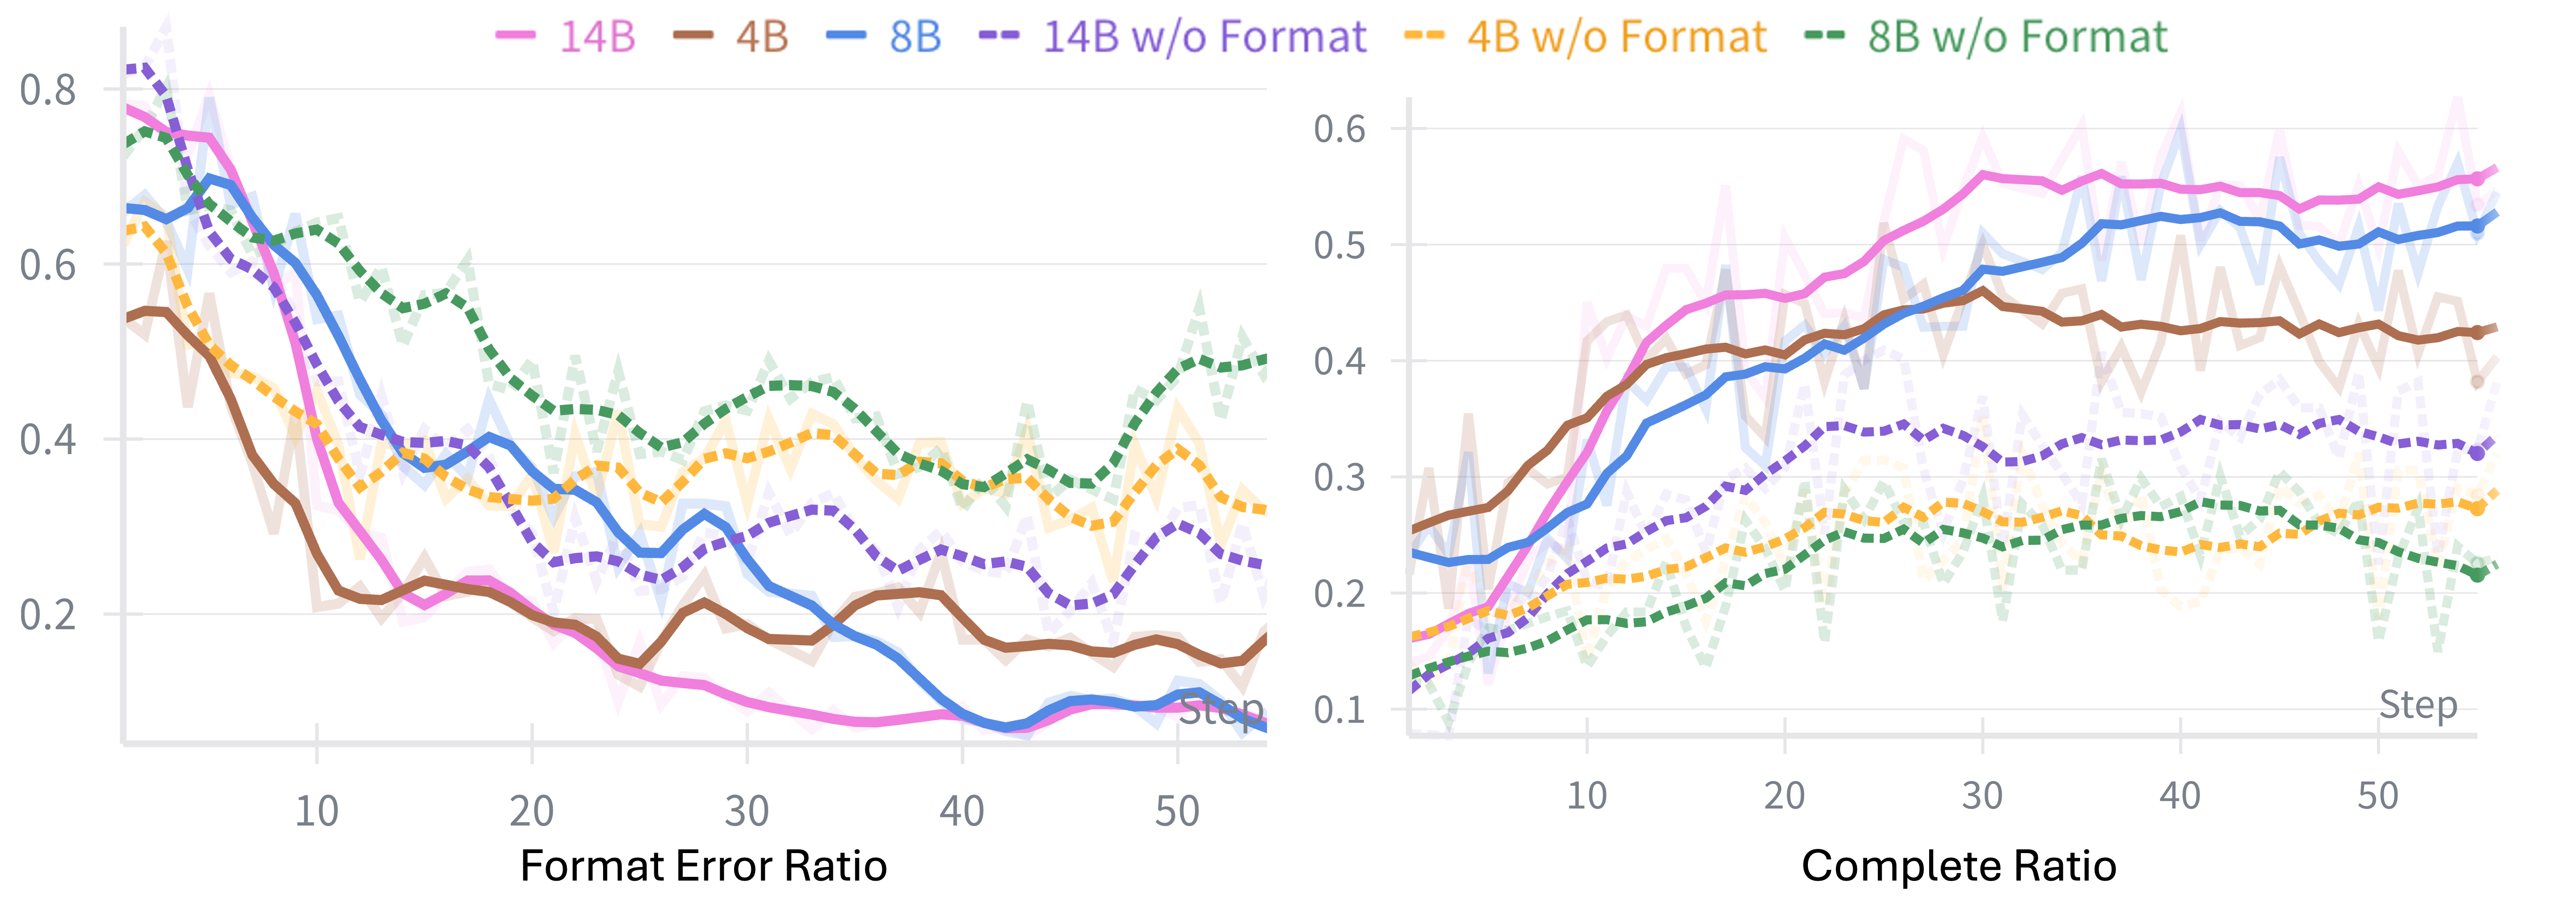
\includegraphics[width=0.8\columnwidth]{figures/step_reward_cmp.png}
    \caption{Format error ratio comparison of \synth. ``w/o Format'' means disabling the step-level format correctness reward. 
    }
    \label{fig:format_error_ratio_cmp}
  \end{figure}
  
  

We study the impact of the step-level format correctness reward in Figure~\ref{fig:format_error_ratio_cmp}.
With this reward, agents quickly learn to follow the tool interface contract, and the format error ratio rapidly converges to a low level.
It also improves training efficiency by reducing the average rollout time by about $27\%$.
In contrast, without this reward, the format error ratio remains above $20\%$ even after 50 optimization steps, leading to frequent invalid actions and noisier learning signals.
This degradation further translates into a lower task completion rate, which saturates below $40\%$.
Overall, the step-level format correctness reward improves both agent performance and training efficiency.


\subsection{Case Study for Verification} \label{appendix:case_study_for_verification}
We provide three representative cases in Figures~\ref{fig:case1}, \ref{fig:case2}, and \ref{fig:case3} to illustrate why our code-augmented LLM-as-a-Judge is more robust than either rigid code-only verification or LLM-only judging from agent trajectories.
For the first case (Fig.~\ref{fig:case1}), the task is a clean, database-grounded query: the agent calls the correct tool to retrieve the full bid history of the item and summarize the findings; the verifier can deterministically confirm these statistics from the underlying state/returned records, and the judge aligns, illustrating the ideal regime where structured verification evidence is decisive. 
For the second case (Fig.~\ref{fig:case2}), the environment exhibits an imperfection when the agent tries to create a routine; a strict code-only verifier that expects a state delta would incorrectly flag failure because the initial and final snapshots appear identical, yet the trajectory shows an idempotent success path, and the code-augmented judge uses this context to correctly mark \texttt{Completed}, reducing false negatives under transient tool/infrastructure issues. 
For the last case (Fig.~\ref{fig:case3}), an API/tool calling error misleads the agent into creating a duplicate event and then adding the session under the wrong event ID; tool calls succeed locally so a judge without verifier grounding could be fooled into marking \texttt{Completed}, but the verifier reveals the real target event remains unchanged, enabling the code-augmented judge to identify a wrong operation and correctly reject the spurious success claim.

Overall, the key theme is that synthetic interactive environments are imperfect: transient tool failures, idempotent tasks, and ambiguous tool calling behaviors can all break the assumptions of rigid verification.
Our design mitigates this by letting the verifier extract \emph{structured evidence} from database snapshots and rule-based checks, while the judge reasons over \emph{trajectory context} to resolve ambiguity and reduce both false negatives and false positives.





\begin{figure}
    \centering
    \begin{minipage}{0.48\columnwidth}
        \centering
        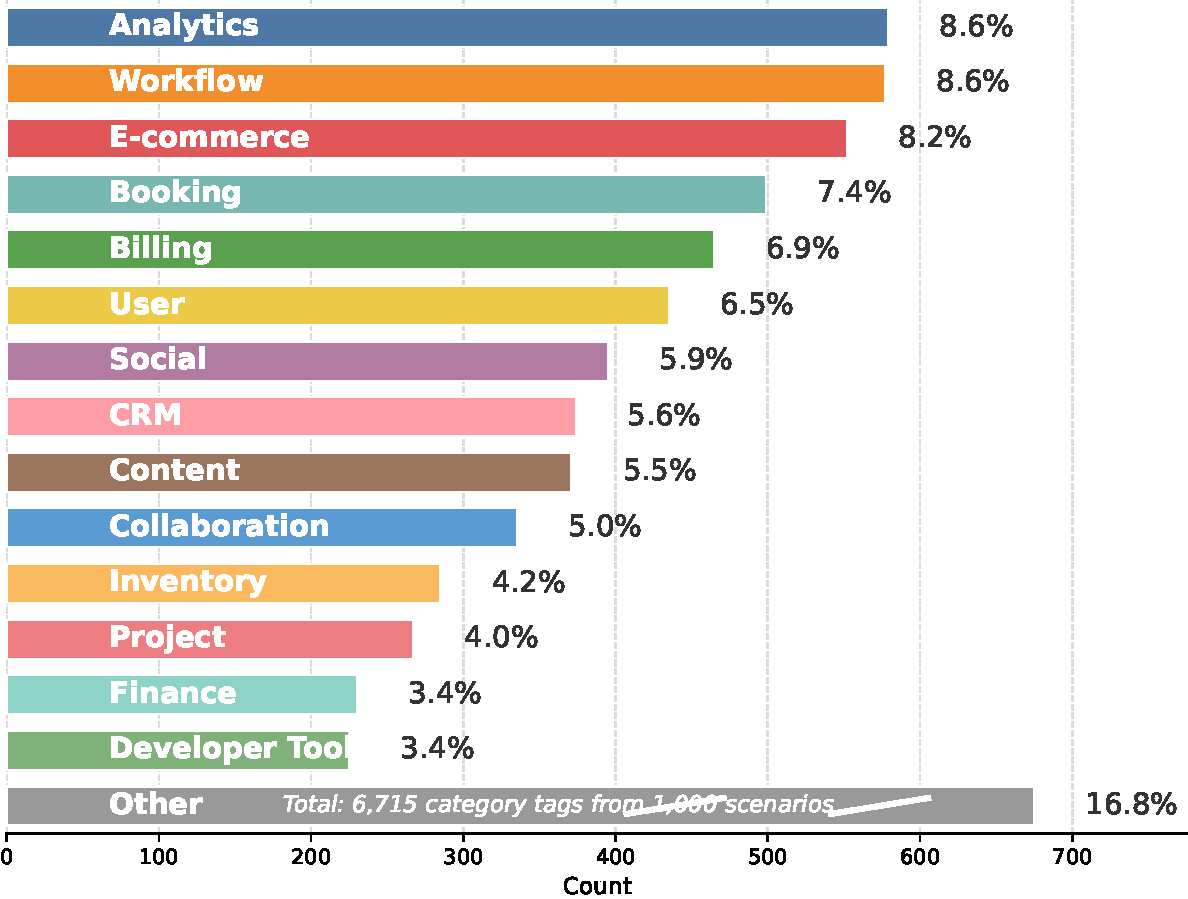
\includegraphics[width=\linewidth]{figures/env_category_distribution.pdf}
        \caption{Distribution of synthesized scenarios of \synth.}
        \label{fig:domain_distribution}
    \end{minipage}
    \hfill
    \begin{minipage}{0.48\columnwidth}
        \centering
        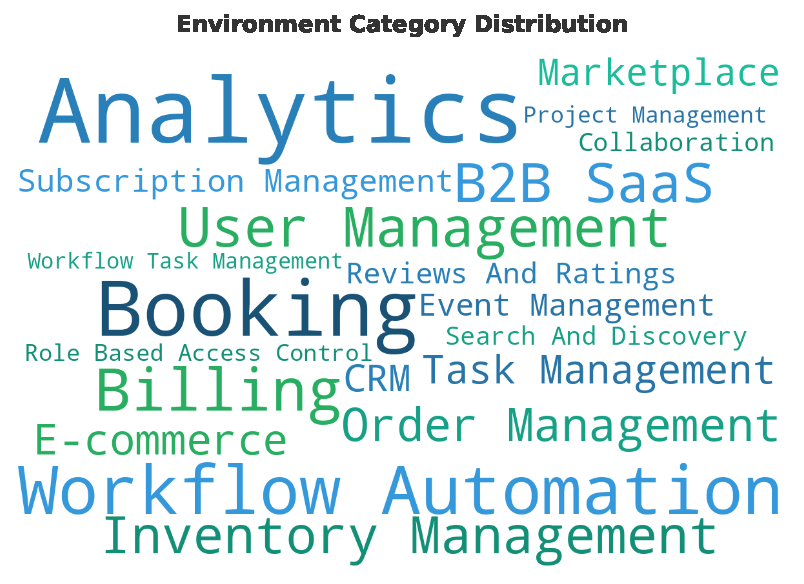
\includegraphics[width=\linewidth]{figures/env_category_wordcloud.pdf}
        \caption{Wordcloud of the scenario descriptions of \synth.}
        \label{fig:wordcloud}
    \end{minipage}
\end{figure}

\begin{figure}
    \centering
    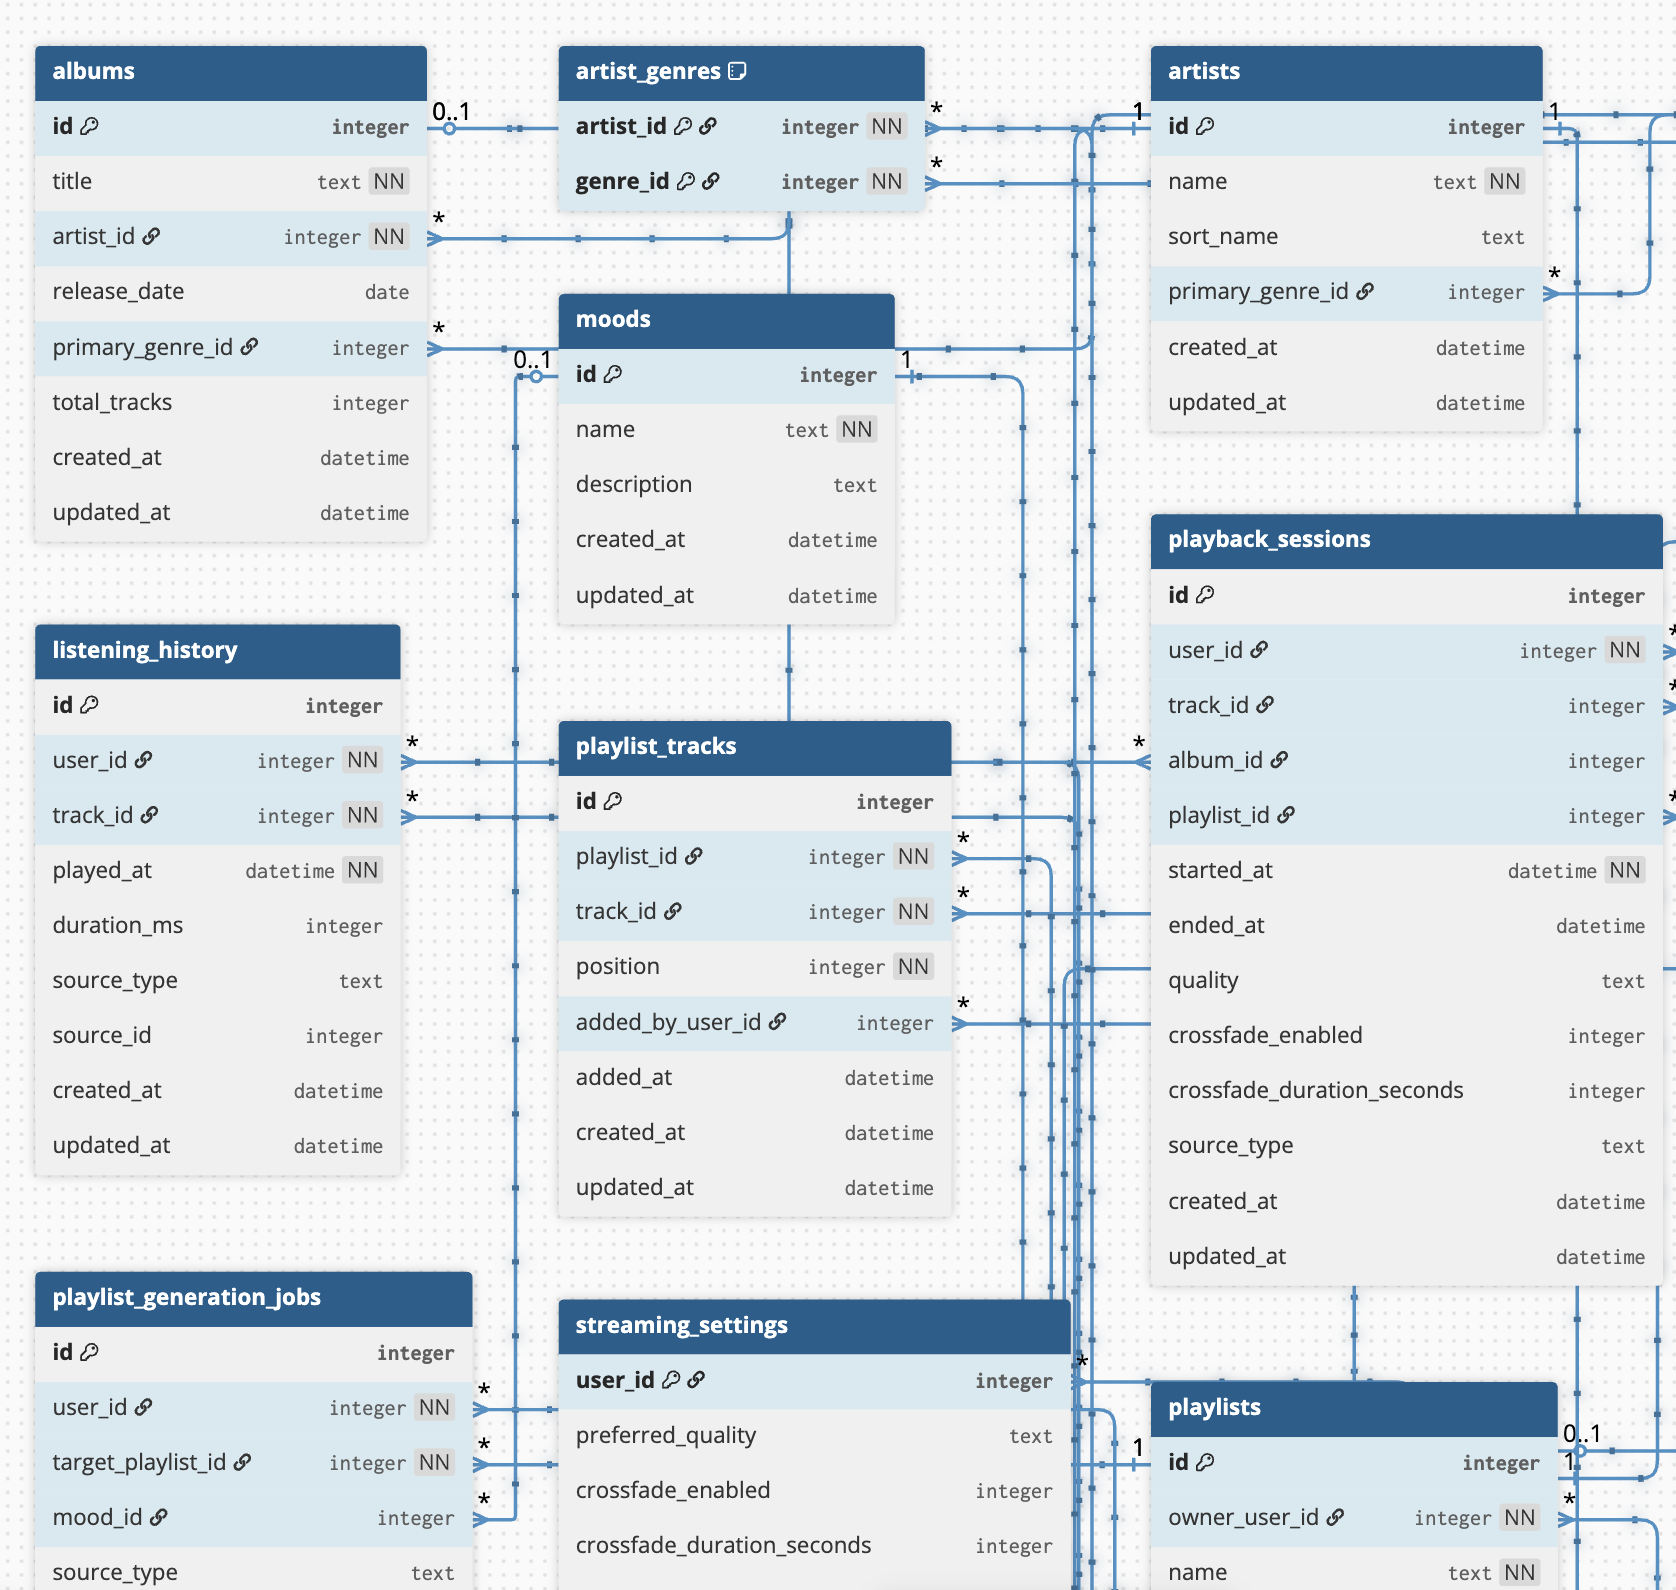
\includegraphics[width=0.7\columnwidth]{figures/database_view.png}
    \caption{Visualization of part of the SQLite database schema of ``Spotify'' environment.}
    \label{fig:database_view}
\end{figure}

\begin{figure*}[t]
    \centering
    \setlength{\fboxrule}{0.8pt}
    \fbox{%
        \begin{minipage}{0.97\textwidth}
        \normalsize
        \vspace{2pt}
        \setlength{\baselineskip}{9pt}

        \texttt{\# MCP Tools}\\[6pt]

        \texttt{You are at a MCP environment. You need to call MCP tools to assist with the user query. At each step, you can only call one function. You have already logged in, and your user id is 1 if required for the MCP tool.}\\[6pt]

        \texttt{You are provided with TWO functions within <tools></tools> XML tags:}\\
        \texttt{<tools>}\\
        \texttt{1. list\_tools}\\
        \texttt{~~~~- Description: List all available MCP tools for the current environment to help you finish the user task.}\\
        \texttt{~~~~- Arguments: None}\\
        \texttt{~~~~- Output: A list of MCP environment-specific tools and their descriptions}\\[4pt]

        \texttt{2. call\_tool}\\
        \texttt{~~~~- Description: Call a MCP environment-specific tool}\\
        \texttt{~~~~- Arguments:}\\
        \texttt{~~~~~~~~- tool\_name: str, required, the tool name in the list\_tools output}\\
        \texttt{~~~~~~~~- arguments: str, required, the arguments for calling <tool\_name>. You must pass a valid JSON string without any markdown fences or additional commentary. This JSON str will be parsed by the tool and executed. You can pass an empty JSON str if no arguments are required by <tool\_name>.}\\
        \texttt{~~~~- Output: The result of the <tool\_name> tool call}\\
        \texttt{</tools>}\\[6pt]

        \texttt{You should always call list\_tools function first to get the available tools, and should only call it once. You should always directly output the answer or summary at the final step instead of calling any function.}\\[6pt]

        \texttt{For each function call, return a json object with function name and arguments within <tool\_call></tool\_call> XML tags:}\\
        \texttt{<tool\_call>}\\
        \texttt{\{"name": <function-name>, "arguments": <args-json-object>\}}\\
        \texttt{</tool\_call>}\\[6pt]

        \texttt{Example Function Call \#1:}\\
        \texttt{<tool\_call>}\\
        \texttt{\{"name": "list\_tools", "arguments": null\}}\\
        \texttt{</tool\_call>}\\[4pt]

        \texttt{Example Function Call \#2:}\\
        \texttt{<tool\_call>}\\
        \texttt{\{"name": "call\_tool", "arguments": \{"tool\_name": "get\_weather", "arguments": "\{"city": "Beijing"\}"\}\}}\\
        \texttt{</tool\_call>}\\[2pt]

        \vspace{1pt}
        \end{minipage}
    }
    \captionsetup{labelformat=default, name=Table}
    \caption{System prompt for agent in MCP environments.}
    \label{fig:agent-system-prompt}
\end{figure*}


\begin{table*}[t]
\centering
\caption{A random sample of 100 generated scenarios from \synth.
The collection includes both synthetic applications and real-world services that represent common enterprise and consumer tool-use patterns.}
\label{tab:scenarios_demo}
\scriptsize
\begin{tabular}{p{5.2cm}p{5.2cm}p{5.2cm}}
\toprule
\textbf{Scenario Name} & \textbf{Scenario Name} & \textbf{Scenario Name} \\
\midrule
ArenaPlay Competitive Gaming Hub & AT\&T & AutoCareLane Service Scheduler \\
AutoGrid Dealer Inventory Manager & Basecamp & Bill.com \\
BlockBridge HOA \& Condo Community Manager & CampusEnroll Admissions Registration Suite & Canva \\
Charles Schwab & CineRealm Digital Cinema & ClaimWise Property \& Auto Insurance Claims Desk \\
ClassBench Music School Scheduling \& Attendance & ClassTrack Micro-LMS & ClinicConnect Multi-Specialty Appointment Center \\
ClinicPaws Veterinary Practice Suite & ClubNest Membership Hub & CodeMentor Classroom LMS \\
CraftBench Custom Manufacturing Job Tracker & DeskQueue IT Support & DevForum Hub (Technical Q\&A Forum) \\
DeviceFleet Cloud Appliance Manager & Discord & Duo Security (Cisco Duo) \\
Eventbrite & EventHarbor Conference \& Session Manager & FleetAxis Commercial Fleet Command \\
Fleetio & FleetPath Manager & FlexDesk Workspace Reservations \\
FlowMesh Workflow Automation Hub & FlowPay Subscription Billing Engine & FlowTrack Team Workflow Hub \\
FormPilot Enterprise Surveys \& Workflows & FundHarbor Retail Investing \& Portfolio Tracker & GhostKitchenOS Virtual Brand Manager \\
GitHub & GiveStream Community Grants Hub & GiveWell-style Donation Portal \\
Gmail & GrantPath Scholarship Application Portal & GreenLedger Utility \& Sustainability Dashboard \\
GuildForge Esports Hub & HelpLane Support Desk & HireBench Coding Graduate Pipeline \\
HireBoard Remote Jobs Marketplace & HomeFlow Smart Device Console & HomeGrid Smart Panel \\
HostEase Property Bookings & InsightLoop Feedback \& NPS Tracker & Jira \\
KitchenGrid Restaurant Ops Hub & LeaseLink Corporate Workspace & ListNest Shared Collections \& Bookmarks \\
LootPlaza Virtual Goods Marketplace & MacroMate Corporate Meal Program Portal & Microsoft 365 (Office) \\
Microsoft Account (Live.com) & Mindbody & NeighborHands Volunteer Network \\
NeighborLink Mutual Aid Exchange & Notion & OpenTable \\
PantryPicks Grocery \& Recipe Wishlist & PawSitter Network \& Booking Hub & PayBridge Merchant Payments Gateway \\
PayStream Merchant Payment Hub & PetCrate Supply Subscriptions & PinHarbor Visual Bookmarks \\
PrepLine Kitchen Display \& Routing & QuickBite Campus Food Ordering & QuickLift Auto Service Booking \\
RegShield Policy Compliance \& Attestation Center & Restaurant Backoffice Pro & Reverb \\
Salesforce & ShelfStack Personal Media Library & SignSure Enterprise E-Signature \& Policy Acknowledgment \\
SitBuddy Pet Sitting \& Home Visit Marketplace & SkinMart Virtual Goods Marketplace & SlotBand Event \& Vendor Scheduler \\
StackList Personal Collections Manager & StockCrate Warehouse Inventory Cloud & Stripe Dashboard \\
SubScript Subscription \& Billing Manager & SubStream Creator Membership Hub & SyncRoom Remote Collaboration Suite \\
TailCart Pet Supplies Marketplace & TalentLoop Recruiting CRM & TeleVisit360 Virtual Care \\
Toast POS & TutorLane Subject Sessions & VendorVault Procurement \& Vendor Portal \\
VenueLane Event Space Booker & VetConnect Telehealth Hub & VolunteerGrid Scheduling \& Shift Manager \\
VolunteerShift Scheduler & WalkLoop Pet Sitting Network & WishCart Social Shopping Lists \\
WishLoom Multi-Store Gift Registry & & \\
\bottomrule
\end{tabular}
\end{table*}

\begin{figure*}[p]
    \centering
    \setlength{\fboxrule}{0.8pt}
    \fbox{%
        \begin{minipage}{0.97\textwidth}
        \small
        \vspace{2pt}
        \setlength{\baselineskip}{8pt}

        \texttt{You are an expert at identifying websites, apps, and digital platforms that are HIGHLY SUITABLE for API environment simulation and database-driven interactions.}\\[4pt]

        \texttt{\#\# KEY PRINCIPLE: Can the data be SYNTHESIZED?}\\
        \texttt{We need platforms where data can be FAKED but still be REALISTIC and USEFUL.}\\[3pt]

        \texttt{\#\#\# Data that CAN be synthesized:}\\
        \texttt{- Numbers: temperatures, prices, quantities, ratings, coordinates, stock prices}\\
        \texttt{- Entities: users, products, orders, bookings, employees, devices, sensors}\\
        \texttt{- Status values: order status, flight status, device state}\\
        \texttt{- Short text: names, titles, addresses, categories, descriptions}\\
        \texttt{- Timestamps: dates, schedules, deadlines, historical records}\\
        \texttt{- Geographic: cities, airports, coordinates (static data)}\\[3pt]

        \texttt{\#\#\# Data that CANNOT be synthesized meaningfully:}\\
        \texttt{- Long articles: news content, blog posts, encyclopedia entries}\\
        \texttt{- Media: actual video/audio content (not metadata)}\\
        \texttt{- AI inference: chatbot responses, ML-based recommendations}\\
        \texttt{- Real search: search engine results with ranking}\\[4pt]

        \texttt{\#\# HIGH Suitability Examples (GENERATE THESE):}\\
        \texttt{E-commerce: CRUD on orders, reviews (products, orders, cart, reviews)}\\
        \texttt{Task Management: CRUD on tasks (tasks, boards, assignments)}\\
        \texttt{Banking/Fintech: CRUD on transactions (accounts, transactions, transfers)}\\
        \texttt{Booking/Reservation: CRUD on reservations (listings, bookings, availability)}\\
        \texttt{Weather Services: Query weather data (locations, forecasts, alerts, history)}\\
        \texttt{Flight/Travel: Search \& book flights (flights, airports, bookings, prices)}\\
        \texttt{Stock Trading: Trade \& portfolio (stocks, trades, portfolio, prices)}\\
        \texttt{IoT/Smart Home: Control devices (devices, sensors, readings, schedules)}\\
        \texttt{Fitness Tracking: Log workouts (workouts, exercises, metrics, goals)}\\
        \texttt{Healthcare: Manage appointments (patients, appointments, records, prescriptions)}\\
        \texttt{HR/Payroll: Manage employees (employees, timesheets, payroll)}\\
        \texttt{CRM/Sales: Manage leads (leads, deals, contacts, activities)}\\
        \texttt{Inventory: Manage stock (products, inventory, warehouses)}\\
        \texttt{Logistics: Track shipments (shipments, packages, routes, status)}\\
        \texttt{Restaurant/Food: Orders \& menu (menu\_items, orders, reservations)}\\
        \texttt{Property/Real Estate: Listings \& viewings (properties, listings, viewings, offers)}\\
        \texttt{Education/LMS: Courses \& grades (courses, enrollments, assignments, grades)}\\
        \texttt{Event Management: Events \& tickets (events, tickets, attendees, venues)}\\[4pt]

        \texttt{\#\# LOW Suitability (AVOID THESE):}\\
        \texttt{News sites (BBC, CNN): Article CONTENT is the product (cannot synthesize meaningful articles)}\\
        \texttt{Wikipedia/Encyclopedia: Article CONTENT is the product (cannot fake knowledge)}\\
        \texttt{Search Engines: Need real search index + ranking (cannot simulate relevance)}\\
        \texttt{AI Assistants (ChatGPT): Need real AI inference (cannot fake AI responses)}\\
        \texttt{Translation (Google Translate): Need real NLP models (cannot fake translations)}\\
        \texttt{Content platforms focus: If CONTENT is core value (metadata is not enough)}\\[4pt]

        \texttt{\#\# MEDIUM Suitability (Focus on CRUD aspects):}\\
        \texttt{YouTube: CAN simulate playlists, subs, comments, channel mgmt; CANNOT simulate actual videos, recommendations}\\
        \texttt{Spotify: CAN simulate playlists, library, following; CANNOT simulate actual audio, music discovery}\\
        \texttt{Reddit: CAN simulate posts (short), comments, votes; CANNOT simulate long-form quality content}\\[4pt]

        \texttt{\#\# Categories to Cover (for diversity):}\\
        \texttt{E-commerce, Booking/Reservation, Task/Project Management, Finance/Banking, Weather/Environmental, Flight/Travel, Stock/Investment,}\\
        \texttt{IoT/Smart Home, Fitness/Health Tracking, Healthcare/Medical, HR/Recruiting, CRM/Sales, Inventory/Warehouse, Logistics/Shipping,}\\
        \texttt{Restaurant/Food, Real Estate, Education/LMS, Event/Ticketing, Legal/Contracts, Subscription Management, Customer Support,}\\
        \texttt{Forms/Surveys, Analytics Dashboards, Fleet Management, Utility Management (electricity, water), Insurance, Pet Services, Automotive}\\[4pt]

        \texttt{\#\# Your Task:}\\
        \texttt{Generate NEW platforms that are HIGHLY SUITABLE where data can be realistically SYNTHESIZED and users perform meaningful CRUD operations.}

        \vspace{1pt}
        \end{minipage}
    }
    \captionsetup{labelformat=default, name=Figure}
    \caption{System prompt for scenario generation (part 1 of 2).}
    \label{fig:gen-scenario-system}
\end{figure*}

\begin{figure*}[p]
    \centering
    \setlength{\fboxrule}{0.8pt}
    \fbox{%
        \begin{minipage}{0.97\textwidth}
        \small
        \vspace{2pt}
        \setlength{\baselineskip}{9pt}

        \texttt{Here are \{num\_examples\} examples of suitable website/app scenarios:}\\[3pt]

        \texttt{\{examples\}}\\[6pt]

        \texttt{---}\\[4pt]

        \texttt{Now generate \{num\_to\_generate\} NEW and DIVERSE website/app/platform scenarios that are DIFFERENT from all examples above.}\\[4pt]

        \texttt{Requirements:}\\
        \texttt{1. Each scenario must be suitable for API environment synthesis (CRUD operations, database interactions)}\\
        \texttt{2. Cover DIFFERENT interaction patterns and industries than the examples}\\
        \texttt{3. Include a mix of: well-known platforms, niche services, B2B tools, mobile apps, and specialized tools}\\
        \texttt{4. The description should emphasize: what entities users can manage, what operations are available, what workflows exist}\\
        \texttt{5. Avoid content-heavy sites, real-time data sites, search engines, AI inference services}\\
        \texttt{6. Each description should be 150-300 words, focusing on actionable features}\\[4pt]

        \texttt{Output format (JSON array, no markdown fences):}\\
        \texttt{[}\\
        \texttt{~~~~\{\{"name": "Platform Name", "url": "example.com", "description": "Description focusing on CRUD operations, entities, and workflows..."\}\},}\\
        \texttt{~~~~...}\\
        \texttt{]}\\[4pt]

        \texttt{Generate exactly \{num\_to\_generate\} new scenarios:}

        \vspace{1pt}
        \end{minipage}
    }
    \captionsetup{labelformat=default, name=Figure}
    \caption{User prompt template for scenario generation (part 2 of 2).}
    \label{fig:gen-scenario-user}
\end{figure*}

\begin{figure*}[p]
    \centering
    \setlength{\fboxrule}{0.8pt}
    \fbox{%
        \begin{minipage}{0.97\textwidth}
        \normalsize
        \vspace{2pt}
        \setlength{\baselineskip}{9pt}

        \textbf{System Prompt:}\\[2pt]
        \texttt{You are an expert in web automation and user task analysis. Your job is to generate realistic, diverse user tasks for scenarios.}\\[6pt]

        \textbf{User Prompt:}\\[2pt]
        \texttt{Generate \{num\_tasks\} realistic and diverse user tasks for the following scenario.}\\[3pt]

        \texttt{Note: A scenario can be a website (e.g., Amazon), a mobile app (e.g., Uber), or a collection of tools and services that provide related}\\
        \texttt{functionality (e.g., Google Workspace combining Gmail, Drive, Calendar). This is part of an automatic environment synthesis pipeline}\\
        \texttt{where we generate executable tool-use environments.}\\[4pt]

        \texttt{Scenario: \{scenario\_name\}}\\
        \texttt{Description: \{scenario\_description\}}\\[4pt]

        \texttt{Requirements:}\\
        \texttt{1. Tasks should be specific and actionable}\\
        \texttt{2. Cover different user scenarios (beginner to advanced)}\\
        \texttt{3. Include both common and less common use cases}\\
        \texttt{4. Tasks should be practical and realistic}\\
        \texttt{5. Each task should be a single sentence including all the necessary information to complete. For example, if the task is to post}\\
        \texttt{~~~a tweet, the task should include the tweet content. If the task is querying the weather, the task should include a specific location.}\\
        \texttt{6. If the scenario typically requires authentication, EXCLUDE any authentication, login, logout, or user registration tasks - assume}\\
        \texttt{~~~the user is already logged in}\\
        \texttt{7. If the scenario typically requires authentication, all tasks should be from the perspective of the current authenticated user}\\
        \texttt{8. Return ONLY a JSON array of tasks, no additional text or annotations}\\
        \texttt{9. The scenario is a simplified version providing API endpoints for task completion. Avoid generating tasks that require direct}\\
        \texttt{~~~user interaction such as download a file, open a page, etc.}\\[4pt]

        \texttt{Examples:}\\
        \texttt{- For scenario ``Amazon'', a task could be ``Search for 'laptop' and add the cheapest result to the cart''}\\
        \texttt{- For scenario ``Reddit'', a task could be ``Get the number of posts in the 'r/python' subreddit''}\\
        \texttt{- For scenario ``Expedia'', a task could be ``Book a flight from New York to London on October 1st''}\\
        \texttt{- For scenario ``Twitter/X'', a task could be ``Post a tweet with a photo, add alt text ``Sunset over the city'', include the hashtag}\\
        \texttt{~~~\#Photography, and mention @Adobe.''}\\
        \texttt{- For scenario ``LinkedIn'', a task could be ``Update my profile headline to 'Senior Data Analyst | SQL, Python, Tableau' and rewrite}\\
        \texttt{~~~the About section to a concise 3-paragraph summary highlighting business impact.''}\\
        \texttt{- For scenario ``Facebook'', a task could be ``Share your latest post to your friend list.''}\\
        \texttt{- For scenario ``Google Maps'', a task could be ``Get 5 most popular restaurants in San Francisco.''}\\[4pt]

        \texttt{Output format:}\\
        \texttt{\{}\\
        \texttt{~~~~``tasks'': [}\\
        \texttt{~~~~~~~~``Task 1 description'',}\\
        \texttt{~~~~~~~~``Task 2 description'',}\\
        \texttt{~~~~~~~~...}\\
        \texttt{~~~~~~~~``Task \{num\_tasks\} description''}\\
        \texttt{~~~~]}\\
        \texttt{\}}

        \vspace{1pt}
        \end{minipage}
    }
    \captionsetup{labelformat=default, name=Figure}
    \caption{Prompts for task generation given a scenario description.}
    \label{fig:gen-task}
\end{figure*}

\begin{figure*}[p]
    \centering
    \setlength{\fboxrule}{0.8pt}
    \fbox{%
        \begin{minipage}{0.97\textwidth}
        \normalsize
        \vspace{2pt}
        \setlength{\baselineskip}{9pt}

        \textbf{System Prompt:}\\[2pt]
        \texttt{You are an expert database architect specializing in SQLite schema design. Your job is to create complete database schemas that can fully support the given user intentions.}\\[6pt]

        \textbf{User Prompt:}\\[2pt]
        \texttt{Design a complete SQLite database schema to support the following user intentions for a simplified version of \{scenario\_name\}.}\\[3pt]

        \texttt{Note: A scenario can be a website, a mobile app, or a collection of tools and services. This is part of an automatic environment}\\
        \texttt{synthesis pipeline where we generate executable tool-use environments.}\\[4pt]

        \texttt{User Intentions (\{num\_tasks\} tasks):}\\
        \texttt{\{user\_intentions\}}\\[4pt]

        \texttt{Requirements:}\\
        \texttt{1. Create ALL necessary tables to cover all the given user intentions}\\
        \texttt{2. Include proper primary keys, foreign keys, indexes, and constraints}\\
        \texttt{3. Use appropriate data types for SQLite (TEXT, INTEGER, REAL, BLOB)}\\
        \texttt{4. Add timestamps (created\_at, updated\_at) where appropriate}\\
        \texttt{5. Do not include any example records in the DDL statements}\\
        \texttt{6. Only create tables and fields that are necessary to cover all the given user intentions}\\
        \texttt{7. EXCLUDE authentication-related fields like password\_hash, salt, token, session - assume authentication is handled externally}\\
        \texttt{8. If a users table is needed, only include essential profile fields (id, username, email, profile data)}\\
        \texttt{9. All operations will be performed as the authenticated user with user\_id=1}\\
        \texttt{10. Return ONLY valid JSON with DDL statements}\\[4pt]

        \texttt{Output format (without any comments):}\\
        \texttt{\{}\\
        \texttt{~~~~``tables'': [}\\
        \texttt{~~~~~~~~\{}\\
        \texttt{~~~~~~~~~~~~``name'': ``users'',}\\
        \texttt{~~~~~~~~~~~~``ddl'': ``CREATE TABLE users (id INTEGER PRIMARY KEY, username TEXT UNIQUE NOT NULL, email TEXT UNIQUE NOT NULL,}\\
        \texttt{~~~~~~~~~~~~~~~~~~~~~~full\_name TEXT, created\_at DATETIME DEFAULT CURRENT\_TIMESTAMP);'',}\\
        \texttt{~~~~~~~~~~~~``indexes'': [}\\
        \texttt{~~~~~~~~~~~~~~~~``CREATE INDEX idx\_users\_email ON users(email);''}\\
        \texttt{~~~~~~~~~~~~]}\\
        \texttt{~~~~~~~~\}}\\
        \texttt{~~~~]}\\
        \texttt{\}}

        \vspace{1pt}
        \end{minipage}
    }
    \captionsetup{labelformat=default, name=Figure}
    \caption{Prompts for database schema generation given user tasks.}
    \label{fig:gen-db}
\end{figure*}

\begin{figure*}[p]
    \centering
    \setlength{\fboxrule}{0.8pt}
    \fbox{%
        \begin{minipage}{0.97\textwidth}
        \normalsize
        \vspace{2pt}
        \setlength{\baselineskip}{8pt}

        \textbf{System Prompt:}\\[2pt]
        \texttt{You are an expert database engineer and data generator specializing in creating comprehensive test datasets for AI agent task execution.}\\
        \texttt{Your job is to generate realistic, diverse sample data that ensures agents can successfully complete ALL given user tasks through API calls.}\\[3pt]

        \texttt{You must:}\\
        \texttt{- Strictly follow the provided database schema}\\
        \texttt{- Never invent or guess table or column names that are not present in the schema}\\
        \texttt{- Follow the exact output JSON format specified in the user prompt}\\
        \texttt{- Output ONLY the requested JSON, with no extra explanations or surrounding text}\\[6pt]

        \textbf{User Prompt (Part 1/2):}\\[2pt]
        \texttt{Generate comprehensive sample data for a simplified \{scenario\_name\} that FULLY SUPPORTS agent execution of ALL the given user tasks.}\\[3pt]

        \texttt{Note: A scenario can be a website, a mobile app, or a collection of tools and services. This is part of an automatic environment}\\
        \texttt{synthesis pipeline where we generate executable tool-use environments.}\\[4pt]

        \texttt{User Tasks to Support: \{tasks\_list\}}\\
        \texttt{Existing Database Schema: \{database\_schema\}}\\[4pt]

        \texttt{CRITICAL: Schema Compliance Rules (MUST FOLLOW):}\\
        \texttt{1. Carefully read the CREATE TABLE statement for each table to understand all columns, defaults, and autoincrement behavior.}\\
        \texttt{2. When writing INSERT statements, always explicitly list the column names you are inserting into in the parentheses after the table}\\
        \texttt{~~~name. The parentheses MUST contain ONLY valid column names from the schema, no values or literals.}\\
        \texttt{3. All listed column names MUST exist in the schema and be spelled exactly as defined. Never invent, shorten, pluralize, or rename columns.}\\
        \texttt{4. You may only generate INSERT statements for tables that appear in the ``Existing Database Schema'' section. If a table name is not}\\
        \texttt{~~~present in the schema, DO NOT use it.}\\
        \texttt{5. For every INSERT statement, the number of listed columns MUST equal the number of values provided in the VALUES(...) clause.}\\
        \texttt{6. Double-check each INSERT statement: count listed columns, count values, they MUST be equal.}\\
        \texttt{7. For tables with many columns (10+), be extra careful to ensure every listed column has exactly one corresponding value in the}\\
        \texttt{~~~VALUES(...) clause.}\\
        \texttt{8. For special/virtual/FTS/config tables, use exactly the columns defined in their CREATE TABLE (or CREATE VIRTUAL TABLE) statements.}\\
        \texttt{~~~Do NOT add foreign key columns such as *\_id unless they explicitly exist in the schema.}\\[4pt]

        \texttt{Data Generation Strategy:}\\
        \texttt{For EACH task listed above, analyze what data is required and ensure:}\\
        \texttt{1. All entities referenced in the task exist in the database}\\
        \texttt{2. All relationships needed to complete the task are properly established}\\
        \texttt{3. Query results will return meaningful, non-empty data}\\
        \texttt{4. Edge cases and variations are covered for robust testing}

        \vspace{1pt}
        \end{minipage}
    }
    \captionsetup{labelformat=default, name=Figure}
    \caption{Prompts for sample data generation (part 1 of 2).}
    \label{fig:gen-data-1}
\end{figure*}

\begin{figure*}[p]
    \centering
    \setlength{\fboxrule}{0.8pt}
    \fbox{%
        \begin{minipage}{0.97\textwidth}
        \small
        \vspace{2pt}
        \setlength{\baselineskip}{8pt}

        \textbf{User Prompt (Part 2/2):}\\[4pt]

        \texttt{Hard Requirements:}\\
        \texttt{1. You must strictly follow the provided database schema - use EXACT table names, column names, and valid column counts. Do NOT}\\
        \texttt{~~~invent new tables or columns.}\\
        \texttt{2. Generate INSERT statements for ALL tables necessary to support the tasks, but ONLY for tables that exist in the schema.}\\
        \texttt{3. Ensure data integrity: respect foreign key relationships and constraints.}\\
        \texttt{4. Follow SQLite syntax for INSERT statements.}\\
        \texttt{5. Insert data in the correct order to satisfy foreign key constraints.}\\
        \texttt{6. If a users table exists, ALWAYS create user with id=1 as the first entry - this is the current authenticated user.}\\
        \texttt{7. DO NOT include authentication fields like password\_hash, token, session, even if they appear in the schema.}\\
        \texttt{8. For user-owned data (orders, posts, etc.), create MOST data for user\_id=1.}\\
        \texttt{9. For each table in the output, provide a brief reasoning (<= 100 words) in its ``reasoning'' field explaining how that table's insert}\\
        \texttt{~~~statements support the given user tasks and comply with the database schema.}\\
        \texttt{10. Return ONLY valid JSON, no additional text. Do NOT include comments, ellipsis (``...''), or wrap the JSON in backticks or code fences.}\\
        \texttt{11. Each element in ``insert\_statements'' MUST be a single SQL INSERT statement string, ending with a single semicolon, and MUST NOT}\\
        \texttt{~~~~contain multiple statements or any JSON/text before or after the SQL.}\\
        \texttt{12. All items in ``insert\_statements'' MUST be plain strings (SQL statements only), not objects or nested JSON structures.}\\[4pt]

        \texttt{INSERT Statement Format (MANDATORY):}\\
        \texttt{- Always explicitly list the column names you are inserting into in each INSERT statement}\\
        \texttt{- Format: INSERT INTO table\_name (col1, col2, ..., colN) VALUES (val1, val2, ..., valN);}\\
        \texttt{- The number of listed columns MUST equal the number of values}\\
        \texttt{- The parentheses after the table name MUST contain ONLY column names, never literal values}\\
        \texttt{- For NULL values, use NULL (not empty string)}\\
        \texttt{- For boolean columns, use 0 or 1}\\
        \texttt{- For optional columns with defaults or autoincrement primary keys, either include them with a value or omit both the column and the}\\
        \texttt{~~corresponding value from the INSERT}\\[4pt]

        \texttt{Agent Task Coverage Requirements:}\\
        \texttt{1. For SEARCH/FILTER tasks: create diverse data that matches AND does not match search criteria}\\
        \texttt{2. For LIST/GET tasks: create multiple records (at least 5-10) to return meaningful results}\\
        \texttt{3. For CREATE/POST tasks: ensure all referenced entities (users, categories, etc.) exist}\\
        \texttt{4. For UPDATE/PATCH tasks: create existing records that can be modified}\\
        \texttt{5. For DELETE tasks: create expendable records that can be safely deleted}\\
        \texttt{6. For AGGREGATION tasks (count, sum, avg): create sufficient data volume for meaningful statistics}\\
        \texttt{7. For RELATIONSHIP tasks: ensure all foreign key references are valid and queryable}\\[4pt]

        \texttt{Data Quality Requirements:}\\
        \texttt{1. Use realistic values (real product names, proper email formats, realistic prices, etc.)}\\
        \texttt{2. Create temporal diversity (records from different dates/times)}\\
        \texttt{3. Include status variations (active/inactive, pending/completed, etc.)}\\
        \texttt{4. Cover numeric ranges (low/medium/high prices, quantities, ratings)}\\
        \texttt{5. Include text variations (short/long descriptions, different categories)}\\
        \texttt{6. For timestamps, use ISO 8601 format: YYYY-MM-DD HH:MM:SS or datetime('now', '-N days')}\\
        \texttt{7. Create enough data volume to support robust testing}\\[4pt]

        \texttt{Output format: \{``tables'': [\{``table\_name'': ``users'', ``reasoning'': ``Brief explanation...'', ``insert\_statements'': [``INSERT INTO ...'', ...]\}, ...]\}}

        \vspace{1pt}
        \end{minipage}
    }
    \captionsetup{labelformat=default, name=Figure}
    \caption{Prompts for sample data generation (part 2 of 2).}
    \label{fig:gen-data-2}
\end{figure*}

\begin{figure*}[p]
    \centering
    \setlength{\fboxrule}{0.8pt}
    \fbox{%
        \begin{minipage}{0.97\textwidth}
        \footnotesize
        \vspace{2pt}
        \setlength{\baselineskip}{8.5pt}

        \textbf{System Prompt:}\\[2pt]
        \texttt{You are an expert API designer and backend architect. Your job is to design machine-readable RESTful API documentation that can support all the given user tasks based on the existing database schema.}\\[6pt]

        \textbf{User Prompt (Part 1/2):}\\[2pt]
        \texttt{Design a complete, agent-friendly interface specification to support ALL the following tasks for a simplified \{scenario\_name\} based on}\\
        \texttt{the existing database schema. The generated specification will be used to guide the detailed implementation of the interface layer.}\\[3pt]

        \texttt{Note: A scenario can be a website, a mobile app, or a collection of tools and services. This is part of an automatic environment}\\
        \texttt{synthesis pipeline where we generate executable tool-use environments.}\\[4pt]

        \texttt{User Tasks: \{tasks\_list\}}\\
        \texttt{Existing SQLite Database Schema: \{database\_schema\}}\\[4pt]

        \texttt{Hard Requirements:}\\
        \texttt{1. Design ATOMIC API endpoints - each endpoint should perform ONE specific, well-defined operation}\\
        \texttt{2. The API spec MUST be compatible with FastAPI, SQLAlchemy ORM, and Pydantic v2}\\
        \texttt{3. Maximize REUSABILITY - create base CRUD operations that can be composed together to fulfill the given tasks}\\
        \texttt{4. The API MUST fully follow the database schema - explicitly use the exact table names, column names, and relationships from the schema}\\
        \texttt{5. Use RESTful conventions (GET, POST, PUT, DELETE, PATCH) with proper resource paths}\\
        \texttt{6. Group related endpoints logically by resource type}\\
        \texttt{7. Prefer multiple small, composable endpoints over fewer complex endpoints}\\
        \texttt{8. For complex tasks, design individual atomic operations that can be chained together}\\
        \texttt{9. Ensure each endpoint maps directly to one or more tables in the provided database schema}\\
        \texttt{10. DO NOT include any authentication endpoints (login, logout, register, token refresh) - assume user is already authenticated}\\
        \texttt{11. All operations implicitly use the current authenticated user with user\_id=1}\\
        \texttt{12. For user-specific data, always filter by user\_id=1 automatically - do not require user\_id as a parameter}\\
        \texttt{13. Return ONLY valid JSON, no additional text}\\[4pt]

        \texttt{Agent-Friendly Requirements (REQUIRED for every endpoint):}\\
        \texttt{- summary: a one-line purpose (<= 80 chars) - clear and actionable for AI agents}\\
        \texttt{- description: SINGLE LINE (<= 200 chars; no line breaks) - explains what the endpoint does and when to use it}\\
        \texttt{- operation\_id: unique, snake\_case identifier - agents use this to identify and call endpoints programmatically}\\
        \texttt{- tags: logical grouping array (e.g., [``products''], [``orders'']) - helps agents discover related endpoints}\\
        \texttt{- request\_params: complete parameter specifications with type, param\_type (query/path/body), required flag, description, and example}\\
        \texttt{- response: detailed response schema with field types, descriptions, and examples - enables agents to parse and understand responses}\\[4pt]

        \texttt{Request Parameter Requirements:}\\
        \texttt{- Each parameter MUST include: type, param\_type, required, description, example}\\
        \texttt{- param\_type MUST be one of: ``query'', ``path'', ``body''}\\
        \texttt{- Use descriptive names that clearly indicate the parameter's purpose}\\
        \texttt{- Provide realistic examples that demonstrate expected values}

        \vspace{1pt}
        \end{minipage}
    }
    \captionsetup{labelformat=default, name=Figure}
    \caption{Prompts for interface specification generation (part 1 of 2).}
    \label{fig:gen-api-1}
\end{figure*}

\begin{figure*}[p]
    \centering
    \setlength{\fboxrule}{0.8pt}
    \fbox{%
        \begin{minipage}{0.97\textwidth}
        \footnotesize
        \vspace{2pt}
        \setlength{\baselineskip}{8.5pt}

        \textbf{User Prompt (Part 2/2):}\\[4pt]

        \texttt{Response Schema Requirements:}\\
        \texttt{- Define complete response structure with all fields}\\
        \texttt{- Each field MUST include: type, description, example}\\
        \texttt{- For array types, include ``items'' with full field definitions}\\
        \texttt{- Use consistent naming conventions across all endpoints}\\[6pt]

        \texttt{Output format:}\\
        \texttt{\{}\\
        \texttt{~~~~``api\_groups'': [}\\
        \texttt{~~~~~~~~\{}\\
        \texttt{~~~~~~~~~~~~``group\_name'': ``Products'',}\\
        \texttt{~~~~~~~~~~~~``endpoints'': [}\\
        \texttt{~~~~~~~~~~~~~~~~\{}\\
        \texttt{~~~~~~~~~~~~~~~~~~~~``path'': ``/api/products'',}\\
        \texttt{~~~~~~~~~~~~~~~~~~~~``method'': ``GET'',}\\
        \texttt{~~~~~~~~~~~~~~~~~~~~``summary'': ``List all products with optional filters'',}\\
        \texttt{~~~~~~~~~~~~~~~~~~~~``description'': ``Retrieve a paginated list of products. Use this endpoint to browse or search the product catalog.'',}\\
        \texttt{~~~~~~~~~~~~~~~~~~~~``operation\_id'': ``list\_products'',}\\
        \texttt{~~~~~~~~~~~~~~~~~~~~``tags'': [``products''],}\\
        \texttt{~~~~~~~~~~~~~~~~~~~~``request\_params'': \{}\\
        \texttt{~~~~~~~~~~~~~~~~~~~~~~~~``category'': \{}\\
        \texttt{~~~~~~~~~~~~~~~~~~~~~~~~~~~~``type'': ``string'',}\\
        \texttt{~~~~~~~~~~~~~~~~~~~~~~~~~~~~``param\_type'': ``query'',}\\
        \texttt{~~~~~~~~~~~~~~~~~~~~~~~~~~~~``required'': false,}\\
        \texttt{~~~~~~~~~~~~~~~~~~~~~~~~~~~~``description'': ``Filter products by category name'',}\\
        \texttt{~~~~~~~~~~~~~~~~~~~~~~~~~~~~``example'': ``Electronics''}\\
        \texttt{~~~~~~~~~~~~~~~~~~~~~~~~\},}\\
        \texttt{~~~~~~~~~~~~~~~~~~~~~~~~``min\_price'': \{}\\
        \texttt{~~~~~~~~~~~~~~~~~~~~~~~~~~~~``type'': ``float'',}\\
        \texttt{~~~~~~~~~~~~~~~~~~~~~~~~~~~~``param\_type'': ``query'',}\\
        \texttt{~~~~~~~~~~~~~~~~~~~~~~~~~~~~``required'': false,}\\
        \texttt{~~~~~~~~~~~~~~~~~~~~~~~~~~~~``description'': ``Minimum price filter in USD'',}\\
        \texttt{~~~~~~~~~~~~~~~~~~~~~~~~~~~~``example'': 10.0}\\
        \texttt{~~~~~~~~~~~~~~~~~~~~~~~~\}}\\
        \texttt{~~~~~~~~~~~~~~~~~~~~\},}\\
        \texttt{~~~~~~~~~~~~~~~~~~~~``response'': \{}\\
        \texttt{~~~~~~~~~~~~~~~~~~~~~~~~``products'': \{}\\
        \texttt{~~~~~~~~~~~~~~~~~~~~~~~~~~~~``type'': ``array'',}\\
        \texttt{~~~~~~~~~~~~~~~~~~~~~~~~~~~~``items'': \{}\\
        \texttt{~~~~~~~~~~~~~~~~~~~~~~~~~~~~~~~~``id'': \{``type'': ``integer'', ``description'': ``Unique product identifier'', ``example'': 1\},}\\
        \texttt{~~~~~~~~~~~~~~~~~~~~~~~~~~~~~~~~``name'': \{``type'': ``string'', ``description'': ``Product display name'', ``example'': ``iPhone 15 Pro''\},}\\
        \texttt{~~~~~~~~~~~~~~~~~~~~~~~~~~~~~~~~``price'': \{``type'': ``float'', ``description'': ``Product price in USD'', ``example'': 999.99\}}\\
        \texttt{~~~~~~~~~~~~~~~~~~~~~~~~~~~~\}}\\
        \texttt{~~~~~~~~~~~~~~~~~~~~~~~~\}}\\
        \texttt{~~~~~~~~~~~~~~~~~~~~\},}\\
        \texttt{~~~~~~~~~~~~~~~~~~~~``required\_tables'': [``products''],}\\
        \texttt{~~~~~~~~~~~~~~~~~~~~``required\_fields'': \{}\\
        \texttt{~~~~~~~~~~~~~~~~~~~~~~~~``products'': [``id'', ``name'', ``price'', ``category'']}\\
        \texttt{~~~~~~~~~~~~~~~~~~~~\}}\\
        \texttt{~~~~~~~~~~~~~~~~\}}\\
        \texttt{~~~~~~~~~~~~]}\\
        \texttt{~~~~~~~~\}}\\
        \texttt{~~~~]}\\
        \texttt{\}}

        \vspace{1pt}
        \end{minipage}
    }
    \captionsetup{labelformat=default, name=Figure}
    \caption{Prompts for interface specification generation (part 2 of 2).}
    \label{fig:gen-api-2}
\end{figure*}

\begin{figure*}[p]
    \centering
    \setlength{\fboxrule}{0.8pt}
    \fbox{%
        \begin{minipage}{0.97\textwidth}
        \footnotesize
        \vspace{2pt}
        \setlength{\baselineskip}{8pt}

        \textbf{System Prompt:}\\[2pt]
        \texttt{You are an expert FastAPI backend developer specializing in RESTful APIs that are agent-friendly: every endpoint must include clear}\\
        \texttt{OpenAPI metadata, complete request/response typing, and machine-readable docs. You generate clean, executable FastAPI endpoint}\\
        \texttt{implementations from an API specification and a SQLite database schema. You strictly follow the user prompt's constraints and return output}\\
        \texttt{in the exact required format.}\\[6pt]

        \textbf{User Prompt (Part 1/3):}\\[2pt]
        \texttt{Generate a single, fully self-contained interface implementation (one Python file using FastAPI and exposed via MCP) that simulates a}\\
        \texttt{simplified version of \{scenario\_name\} based on the provided interface specification and database schema.}\\[3pt]

        \texttt{Note: A scenario can be a website, a mobile app, or a collection of tools and services. This is part of an automatic environment}\\
        \texttt{synthesis pipeline where we generate executable tool-use environments.}\\[4pt]

        \texttt{Assumptions:}\\
        \texttt{- Python version: \{PYTHON\_VERSION\}}\\
        \texttt{- FastAPI version compatible with Pydantic v2 (do NOT use v1-only features such as `orm\_mode` in Config)}\\[3pt]

        \texttt{API Specification: \{api\_spec\}}\\
        \texttt{Database Schema: \{database\_schema\}}\\[4pt]

        \texttt{Environment \& Configuration Requirements:}\\
        \texttt{- Import os and read the SQLite database URL from environment variable `DATABASE\_PATH`}\\
        \texttt{- If `DATABASE\_PATH` is not set or empty, default to: sqlite:///xxxx.db}\\
        \texttt{- In the uvicorn entry point, read HOST from environment variable `HOST` (default to ``127.0.0.1'' if not set)}\\
        \texttt{- In the uvicorn entry point, read PORT from environment variable `PORT` (default to 8000 if not set), and cast it to int}\\[3pt]

        \texttt{SQLAlchemy Setup Requirements:}\\
        \texttt{- Use SQLAlchemy ORM with declarative\_base for all tables}\\
        \texttt{- Database URL: use the value of DATABASE\_PATH (or the default described above). The DATABASE\_PATH is a complete URL so do not add}\\
        \texttt{~~any prefixes (e.g., sqlite://) or suffixes to the URL}\\
        \texttt{- Create engine and SessionLocal (sessionmaker) for database sessions}\\
        \texttt{- Define Base = declarative\_base() for ORM inheritance}\\
        \texttt{- Define ORM models for every table present in the database schema (no extra tables/columns)}\\
        \texttt{- Call Base.metadata.create\_all(engine) after all ORM models are defined}\\
        \texttt{- NEVER define ORM attributes named `metadata`, `query`, or `query\_class`. If the schema has a column with one of these names, use a}\\
        \texttt{~~safe Python attribute name with a trailing underscore (e.g. `metadata\_`) and map it to the real column name via Column(``metadata'', ...)}\\
        \texttt{- Do NOT define any other ORM class attribute that conflicts with SQLAlchemy declarative internals}\\
        \texttt{- When there are multiple foreign key paths between two tables, either:}\\
        \texttt{~~- specify relationship(..., foreign\_keys=[...]) explicitly to avoid AmbiguousForeignKeysError, OR}\\
        \texttt{~~- omit the relationship entirely and access related rows via explicit queries instead of relationship()}\\
        \texttt{- When importing from SQLAlchemy, only use standard, public symbols that actually exist and are needed. Do NOT import or reference}\\
        \texttt{~~non-existent or internal symbols such as `PRIMARY\_KEY\_CONSTRAINT` or any other invented uppercase constants}\\
        \texttt{- Import ORM-related helpers from sqlalchemy.orm (for example: declarative\_base, relationship, sessionmaker). Do not import ORM}\\
        \texttt{~~internals from sqlalchemy.\_\_init\_\_}

        \vspace{1pt}
        \end{minipage}
    }
    \captionsetup{labelformat=default, name=Figure}
    \caption{Prompts for interface implementation generation (part 1 of 3).}
    \label{fig:gen-env-1}
\end{figure*}

\begin{figure*}[p]
    \centering
    \setlength{\fboxrule}{0.8pt}
    \fbox{%
        \begin{minipage}{0.97\textwidth}
        \footnotesize
        \vspace{2pt}
        \setlength{\baselineskip}{8pt}

        \textbf{User Prompt (Part 2/3):}\\[4pt]

        \texttt{Hard Requirements:}\\
        \texttt{1. Implement EVERY endpoint from the API spec with COMPLETE, working code. The API spec is for reference only. The source of truth is}\\
        \texttt{~~~the database schema.}\\
        \texttt{2. Follow the API spec as closely as possible: paths, HTTP methods, parameters (query/path/body), and response formats.}\\
        \texttt{3. Follow the EXACT database schema: correct table names, columns, types, and foreign keys; do not invent tables or columns.}\\
        \texttt{4. All endpoint handler functions MUST be async and self-contained.}\\
        \texttt{5. Use ONLY SQLAlchemy ORM (no raw SQL).}\\
        \texttt{6. User-specific operations MUST implicitly filter by user\_id=1 where applicable.}\\
        \texttt{7. Session lifecycle per endpoint:}\\
        \texttt{~~~- session = SessionLocal() at the start}\\
        \texttt{~~~- For INSERT/UPDATE/DELETE call session.commit()}\\
        \texttt{~~~- session.close() before returning}\\
        \texttt{8. No placeholders; write complete, executable code. Do NOT create dummy or placeholder endpoints.}\\
        \texttt{9. Path parameters in routes (e.g., /api/products/\{product\_id\}) MUST appear as function parameters.}\\
        \texttt{10. STRICTLY PROHIBITED in the code: comments, try/except, error handling, validation beyond types, HTTPException, JSONResponse,}\\
        \texttt{~~~~global exception handlers, duplicate route registration for the same path and HTTP method, references to undefined models/fields/tables,}\\
        \texttt{~~~~schema-external FTS or helper tables, or any dynamic/introspective tricks to construct response models.}\\
        \texttt{11. Booleans must be real bool fields in Pydantic responses, not 0/1.}\\
        \texttt{12. The FastAPI app must be defined BEFORE any route decorators.}\\
        \texttt{13. Include the uvicorn entry point at the end, using HOST and PORT from environment variables:}\\[2pt]
        \texttt{~~~~if \_\_name\_\_ == ``\_\_main\_\_'':}\\
        \texttt{~~~~~~~~import uvicorn, os}\\
        \texttt{~~~~~~~~host = os.getenv(``HOST'', ``127.0.0.1'')}\\
        \texttt{~~~~~~~~port = int(os.getenv(``PORT'', ``8000''))}\\
        \texttt{~~~~~~~~uvicorn.run(app, host=host, port=port)}\\[2pt]
        \texttt{14. The generated Python file MUST be valid Python \{PYTHON\_VERSION\} with no syntax errors. Do NOT use Python reserved keywords as}\\
        \texttt{~~~~function parameter names or keyword argument names. If a database column or API field name is a Python keyword (e.g., ``return'',}\\
        \texttt{~~~~``class'', ``global''), use a safe Python identifier with a trailing underscore (e.g., return\_) and map it to the real column name or JSON}\\
        \texttt{~~~~field via Column(``return'', ...) or Field(..., alias=``return'').}\\
        \texttt{15. There MUST be exactly one route function for each (path, HTTP method) pair. Do NOT declare multiple handlers for the same path}\\
        \texttt{~~~~and HTTP method, even temporarily.}\\[4pt]

        \texttt{Pydantic Model Requirements (Pydantic v2):}\\
        \texttt{- Import from Pydantic v2 (e.g., from pydantic import BaseModel, Field, ConfigDict)}\\
        \texttt{- Define request and response models for ALL endpoints}\\
        \texttt{- Use Field for EVERY field with both description and example}\\
        \texttt{- The response\_model specified in each route decorator MUST exactly match what the function returns}\\
        \texttt{- The response\_model argument in each route decorator MUST be a direct reference to a concrete Pydantic BaseModel subclass defined in}\\
        \texttt{~~this file (for example, MyResponseModel, or List[MyResponseModel]), NOT a dynamically computed or introspected expression. Do NOT}\\
        \texttt{~~use \_\_annotations\_\_, \_\_mro\_\_, .\_\_class\_\_, metaclasses, or any other tricks to generate a response\_model}\\
        \texttt{- Endpoint return type annotations MUST be consistent with the response\_model (e.g., MyResponseModel, List[MyResponseModel]) and MUST}\\
        \texttt{~~be valid Pydantic field types. Do NOT use Union[...] return types, Response types, or mixtures like Union[Response, dict, None]}

        \vspace{1pt}
        \end{minipage}
    }
    \captionsetup{labelformat=default, name=Figure}
    \caption{Prompts for interface implementation generation (part 2 of 3).}
    \label{fig:gen-env-2}
\end{figure*}

\begin{figure*}[p]
    \centering
    \setlength{\fboxrule}{0.8pt}
    \fbox{%
        \begin{minipage}{0.97\textwidth}
        \footnotesize
        \vspace{2pt}
        \setlength{\baselineskip}{8pt}

        \textbf{User Prompt (Part 3/3):}\\[4pt]

        \texttt{- When returning ORM objects, configure models for Pydantic v2 using model\_config, for example:}\\[2pt]
        \texttt{~~~~class SomeModel(BaseModel):}\\
        \texttt{~~~~~~~~model\_config = ConfigDict(from\_attributes=True)}\\
        \texttt{~~~~~~~~...}\\[2pt]
        \texttt{- Do NOT use the old Pydantic v1 Config with orm\_mode = True}\\
        \texttt{- Do NOT use Annotated or other advanced type tricks that might cause unevaluable type annotations}\\
        \texttt{- Use ONLY standard typing types: int, float, str, bool, Optional[T], List[T], Dict[str, T]}\\
        \texttt{- Field names MUST NEVER be identical (case-sensitive or case-insensitive) to the name of their own type annotation. If it is required}\\
        \texttt{~~by the API spec or database schema, always choose a different snake\_case field name (e.g. `schedule\_date: date`, `event\_datetime:}\\
        \texttt{~~datetime`), and configure a serialization alias, for example: `schedule\_date: date = Field(..., serialization\_alias=``date'', ...)`}\\
        \texttt{- Ensure that no Pydantic field name clashes with a type name or class name used in the same module}\\[4pt]

        \texttt{Agent-Friendly Enhancements (REQUIRED on every endpoint decorator):}\\
        \texttt{- summary: a one-line purpose (<= 80 chars)}\\
        \texttt{- description: SINGLE LINE (<= 200 chars; no line breaks)}\\
        \texttt{- tags: logical grouping array (e.g., [``products''], [``orders''])}\\
        \texttt{- operation\_id: unique, snake\_case identifier}\\
        \texttt{- response\_model: a concrete Pydantic model class (or typing such as List[Model]) that directly corresponds to the returned value}\\[4pt]

        \texttt{Code Style (MANDATORY):}\\
        \texttt{- app = FastAPI(...) MUST appear before any @app.get/post/put/patch/delete decorators}\\
        \texttt{- Use Query/Path/Body/Depends from fastapi where appropriate}\\
        \texttt{- Use relationship for ORM relations only when they are unambiguous OR explicitly specify foreign\_keys to avoid SQLAlchemy}\\
        \texttt{~~AmbiguousForeignKeysError}\\
        \texttt{- For SELECT: session.query(Model).filter(...).all()/first()}\\
        \texttt{- For INSERT: session.add(...); session.commit()}\\
        \texttt{- For UPDATE: fetch the ORM objects, modify attributes, then session.commit()}\\
        \texttt{- For DELETE: session.delete(obj); session.commit()}\\
        \texttt{- Return Python dicts/lists or Pydantic models that conform exactly to the declared response\_model}\\
        \texttt{- Do NOT use Python reserved keywords as attribute names, function parameters, or keyword argument names. If the schema or API}\\
        \texttt{~~uses such names, use a safe Python name with a trailing underscore and map it via Column(``name'', ...) or Field(..., alias=``name'')}\\
        \texttt{- No comments, no exception handlers, no defensive programming, no placeholder code, and no dynamic hacks around FastAPI or Pydantic}\\[4pt]

        \texttt{Output Format (CRITICAL):}\\
        \texttt{- You MUST return ONLY complete and valid Python source code of the FastAPI app}\\
        \texttt{- The response MUST consist of Python code only. Do NOT include any Markdown, prose, explanations, JSON wrappers, keys, or code fences}\\
        \texttt{- Do NOT wrap the code in JSON. Do NOT add any outer structure. The response itself is the file content}\\
        \texttt{- The FIRST line of your response MUST be a valid Python statement such as `import` or `from` (e.g. `import os` or `from fastapi import FastAPI`)}\\
        \texttt{- Do NOT escape newlines. Output the code exactly as it would appear in a .py file}\\
        \texttt{- If you include ANY non-Python text (such as ``Here is the code:'', backticks, or JSON), the output will be INVALID}\\
        \texttt{- Your entire reply must be a single, self-contained Python module that can be saved directly as a .py file and executed}\\[4pt]

        \texttt{Reminder:}\\
        \texttt{- Use only entities present in the provided database schema. The API spec is only for reference. If the API spec conflicts with the database}\\
        \texttt{~~schema, prioritize the database schema. If following the API spec as written would cause bugs, you MUST use the database schema as}\\
        \texttt{~~the source of truth. Prioritize making the code executable without errors over following the API spec text}\\
        \texttt{- Ensure all endpoints run without undefined names, missing imports, or missing models}\\
        \texttt{- Ensure the code creates the SQLite database specified by the environment variable DATABASE\_PATH on first run and successfully serves}\\
        \texttt{~~all endpoints with the specified response models}

        \vspace{1pt}
        \end{minipage}
    }
    \captionsetup{labelformat=default, name=Figure}
    \caption{Prompts for interface implementation generation (part 3 of 3).}
    \label{fig:gen-env-3}
\end{figure*}

\begin{figure*}[t]
    \centering
    \setlength{\fboxrule}{0.8pt}
    \fbox{%
        \begin{minipage}{0.97\textwidth}
        \small
        \vspace{2pt}
        \setlength{\baselineskip}{9pt}

        \texttt{\textbf{[System Prompt]}}\\[3pt]
        \texttt{You are an expert Python and SQL developer. Your job is to generate Python code that uses SQLite queries to verify if a user task was completed successfully. You only output UTF-8 encoded strings and English text.}\\[6pt]

        \texttt{\textbf{[User Prompt]}}\\[3pt]
        \texttt{You need to generate a Python function with SQLite queries to collect useful information from the given databases to verify if a user task was completed. You are provided with the environment name, the user task to verify, the database schema, and the initial database state.}\\[6pt]

        \texttt{Simplified API Server Name: \{scenario\}}\\
        \texttt{User Task to Verify: \{task\}}\\
        \texttt{Database Dump (Initial State, before the agent takes any action): \{db\_dump\}}\\[6pt]

        \texttt{---}\\[3pt]
        \texttt{\#\#\# Requirements}\\
        \texttt{1. Generate a complete Python function that takes initial\_db\_path and final\_db\_path as parameters.}\\
        \texttt{2. The function should connect to the SQLite database and execute queries to return useful information to assist another LLM to judge the task completion.}\\
        \texttt{3. You can use complex SQLite query combinations and Python logic. The function must return a dictionary containing useful information for judging task completion.}\\
        \texttt{4. The function and queries should follow the database dump. Do not invent new tables or columns.}\\
        \texttt{5. Use the sqlite3 library, and import any other libraries you need.}\\
        \texttt{6. You will be provided with two database states: the initial state and the final state after agent execution. Use the initial state to compare with the final state.}\\
        \texttt{7. You must NOT modify the databases in any way. You can only read from them.}\\
        \texttt{8. Ensure the returned dictionary can be JSON serialized. Use only string, int, float, bool, list, and dict types.}\\
        \texttt{9. You must output a dictionary including: reasoning, python\_code, function\_name, success\_criteria, failure\_criteria.}\\[6pt]
        \texttt{\#\#\# Example Structure}\\[3pt]
        \texttt{def verify\_task(initial\_db\_path: str, final\_db\_path: str) -> dict:}\\
        \texttt{~~~~import sqlite3}\\[2pt]
        \texttt{~~~~conn\_initial = sqlite3.connect(initial\_db\_path)}\\
        \texttt{~~~~conn\_final = sqlite3.connect(final\_db\_path)}\\[2pt]
        \texttt{~~~~\# Query initial and final database states}\\
        \texttt{~~~~\# Compare states to extract task-relevant signals}\\
        \texttt{~~~~\# ...}\\[2pt]
        \texttt{~~~~conn\_initial.close()}\\
        \texttt{~~~~conn\_final.close()}\\[2pt]
        \texttt{~~~~return \{}\\
        \texttt{~~~~~~~~\# Return any valuable data to help determine task completion.}\\
        \texttt{~~~~~~~~\# Ensure this dictionary can be JSON serialized.}\\
        \texttt{~~~~\}}\\[6pt]

        \texttt{---}\\[3pt]
        \texttt{\#\#\# Output Format (must be valid JSON, no markdown fences)}\\
        \texttt{\{}\\
        \texttt{~~"reasoning": "Explanation of why the function can verify task success or failure",}\\
        \texttt{~~"python\_code": "Complete Python function code as a string",}\\
        \texttt{~~"function\_name": "verify\_task",}\\
        \texttt{~~"success\_criteria": "Description of expected results indicating task success",}\\
        \texttt{~~"failure\_criteria": "Description of expected results indicating task failure"}\\
        \texttt{\}}\\[3pt]

        \vspace{1pt}
        \end{minipage}
    }
    \captionsetup{labelformat=default, name=Table}
    \caption{Prompt for verification code generation used for providing verification signals from the database states.}
    \label{tab:verification-prompt-2}
\end{figure*}

\begin{figure*}[t]
    \centering
    \setlength{\fboxrule}{0.8pt}
    \fbox{%
        \begin{minipage}{0.97\textwidth}
        \small
        \vspace{2pt}
        \setlength{\baselineskip}{9pt}

        \texttt{You are an impartial evaluator for tool-use agent task results with access to database verification. Based on the provided agent trajectory AND the code-based verification results from querying the database, decide the task outcome. The trajectory is generated by an MCP agent interacting with a synthesized environment. The environment provides a set of MCP tools to help the agent complete the task.}\\[6pt]

        \texttt{\#\#\# Input}\\
        \texttt{- task\_json: dict containing the user task, execution budget, actual execution steps, and the agent trajectory.}\\
        \texttt{- verification\_json: dict containing verification code, reasoning, success\_criteria, failure\_criteria, and code execution results that verified the database state changes.}\\[6pt]

        \texttt{\#\#\# Classification Categories}\\
        \texttt{- Completed: all required steps were successfully executed, AND the database state confirms the task was completed.}\\
        \texttt{- Partially Completed: partial progress was made, or the database state shows the task is not fully completed.}\\
        \texttt{- Environment Error: the agent is blocked by MCP server or environment error, e.g., 5xx errors such as ``Internal Server Error'', or the MCP server cannot process valid tool calls.}\\
        \texttt{- Agent Error: the agent made mistakes, used invalid parameters, or failed to complete the user's instruction due to agent-side issues.}\\[6pt]

        \texttt{\#\#\# Priority Order for Classification}\\
        \texttt{1. Completed (trajectory shows success AND database confirms it)}\\
        \texttt{2. Environment Error (blocked by MCP server or environment error)}\\
        \texttt{3. Agent Error (agent-side issues, e.g., invalid tool arguments, hallucination)}\\
        \texttt{4. Partially Completed (everything else unfinished or database state mismatch)}\\[6pt]

        \texttt{\#\#\# Key Considerations}\\
        \texttt{- The verification\_json contains checks performed on the database states before and after agent execution.}\\
        \texttt{- Use the verification code execution results to help judge task completion.}\\
        \texttt{- The verification\_json provides success\_criteria and failure\_criteria describing how to interpret state differences.}\\
        \texttt{- The verification results may be empty, erroneous, or inaccurate. Do not fully rely on them. Comprehensively consider the trajectory information to judge task completion.}\\[6pt]

        \texttt{\#\#\# Output Format (must be valid JSON)}\\
        \texttt{\{}\\
        \texttt{~~"reasoning": "<explanation considering both trajectory and verification results>",}\\
        \texttt{~~"confidence\_score": [<int>, <int>, <int>, <int>],}\\
        \texttt{~~"classification": "<Completed | Partially Completed | Environment Error | Agent Error>",}\\
        \texttt{~~"evidence": \{}\\
        \texttt{~~~~"iterations": <int>,}\\
        \texttt{~~~~"error\_signals": ["<important error messages>"],}\\
        \texttt{~~~~"last\_actions": ["<summaries of last few actions>"],}\\
        \texttt{~~~~"database\_verification": "<summary of database state changes>"}\\
        \texttt{~~\}}\\
        \texttt{\}}\\[3pt]


        \vspace{1pt}
        \end{minipage}
    }
    \captionsetup{labelformat=default, name=Table}
    \caption{Prompt for code-augmented LLM-as-a-Judge verification. The judge receives both the agent trajectory and structured verification signals from database state inspection to provide robust reward signals for RL training.}
    \label{tab:prompt_verify_judge}
\end{figure*}



\lstdefinestyle{apischema}{
	basicstyle=\ttfamily\footnotesize,
	frame=single,
	breaklines=true,
	breakatwhitespace=true,
	columns=fullflexible,
	keepspaces=true,
	showstringspaces=false,
	tabsize=1,
	escapechar=@,
	xleftmargin=0pt,
	xrightmargin=0pt,
	aboveskip=0pt,
	belowskip=0pt,
	framexleftmargin=0pt,
	framexrightmargin=0pt,
	framextopmargin=0pt,
	framexbottommargin=0pt
}

\begin{table}[t]
	\centering
	\caption{Example of interface schema snippet with rich annotations and explicit database constraints. 
	}
	\label{tab:demo_api_schema}
	\small

	\begin{minipage}{0.95\columnwidth}
\begin{lstlisting}[style=apischema]
@\textcolor{blue}{"operation\_id"}@: "get_product_by_id",
@\textcolor{blue}{"request\_params"}@: {"product_id": {"type": "integer", "required": true}},
@\textcolor{blue}{"response"}@: {
  "product": {"id": {"type": "integer"}, "title": {"type": "string"}, ....},
  "aggregates": {"average_rating": {"type": "float"}, ....}, ....},
@\textcolor{blue}{"required\_tables"}@: ["products", "product_aggregates", "product_offers"],
@\textcolor{blue}{"required\_fields"}@: {
  "products": ["id", "title", "category_id", ....], ....}\end{lstlisting}
	\end{minipage}
\end{table}


\begin{table*}[t]
\centering
\caption{Example tasks from three synthesized environments. Each task requires multiple tool calls, conditional logic, or complex filtering, demonstrating the diversity and complexity of our generated tasks.}
\label{tab:tasks_demo}
\small
\renewcommand{\arraystretch}{1.3}
\begin{tabular}{@{}m{1.5cm}|p{13.5cm}@{}}
\toprule
\textbf{Scenario} & \textbf{Generated Tasks} \\
\midrule
\multirow{5}{*}[-2em]{\shortstack{\textbf{Music}\\\textbf{Streaming}}}
& Create a new playlist named ``Morning Focus 2025'' with the description ``Upbeat but not distracting'' and add the top 10 most popular tracks by ``Daft Punk'' to it. \\
\cmidrule(l){2-2}
& Generate a personalized playlist of 30 songs based on my recent listening history that match the ``chill'' mood and save it as ``Chill Evening Mix''. \\
\cmidrule(l){2-2}
& Create a collaborative playlist named ``Road Trip to Yosemite'' and add the top 5 rock tracks from the 1990s plus the top 5 pop tracks from the 2010s. \\
\midrule
\multirow{5}{*}[-2em]{\shortstack{\textbf{E-commerce}\\\textbf{Platform}}}
& Search for ``wireless noise cancelling headphones'', sort results by average customer rating, and add the top-rated item under \$200 to my cart in quantity 1. \\
\cmidrule(l){2-2}
& Locate my order for ``Instant Pot Duo 7-in-1'' placed within the last 6 months and initiate a return request selecting ``Item defective or doesn't work'' as the reason and requesting a refund to my original payment method. \\
\cmidrule(l){2-2}
& Subscribe to a ``household paper towels'' product with at least a 4-star rating using Subscribe \& Save, delivering a 12-roll pack every 2 months to my default address. \\
\midrule
\multirow{5}{*}[-2.5em]{\shortstack{\textbf{Travel}\\\textbf{Booking}}}
& Create and save a multi-destination trip itinerary that includes a hotel in Rome (Italy) from August 5--8, 2025 and a hotel in Florence (Italy) from August 8--11, 2025 for 2 adults, choosing mid-range properties (3 or 4 stars) with guest ratings of at least 8.5. \\
\cmidrule(l){2-2}
& Search for vacation packages that bundle hotel and flight from Berlin (BER) to Barcelona (BCN) for April 12--17, 2025 for 2 adults, and return the cheapest package that includes at least a 4-star hotel within 2 km of the city center. \\
\cmidrule(l){2-2}
& Search for pet-friendly apartments in Lisbon, Portugal for a one-month stay from January 5, 2026 to February 5, 2026 for 2 adults and 1 child with a budget of at most \texteuro 80 per night, and return the top three options sorted by guest rating. \\
\bottomrule
\end{tabular}
\end{table*}


\lstdefinestyle{pythonstyle}{
    language=Python,
    basicstyle=\ttfamily\scriptsize,
    keywordstyle=\color{blue}\bfseries,
    stringstyle=\color{red},
    commentstyle=\color{gray}\itshape,
    numbers=left,
    numberstyle=\tiny\color{gray},
    numbersep=5pt,
    breaklines=true,
    breakatwhitespace=false,
    showstringspaces=false,
    frame=single,
    framesep=2pt,
    xleftmargin=15pt,
    framexleftmargin=15pt,
    tabsize=4,
    columns=flexible,
    keepspaces=true,
    escapeinside={(*@}{@*)},
    literate={\_}{\_}1,
}


\begin{figure*}[t]
\centering
\begin{minipage}{0.97\textwidth}
\begin{lstlisting}[style=pythonstyle, firstnumber=1]
from fastapi import FastAPI, Query, Path, Body
from pydantic import BaseModel, Field, ConfigDict
from typing import Optional, List, Dict
from sqlalchemy import create_engine, Column, Integer, String, DateTime, Date, ForeignKey, Text, UniqueConstraint, Index, Float
from sqlalchemy.orm import declarative_base, relationship, sessionmaker
import os
from datetime import datetime

database_url = os.getenv("DATABASE_PATH", "sqlite:///outputs/databases/spotify.db")
engine = create_engine(database_url, connect_args={"check_same_thread": False} if database_url.startswith("sqlite") else {})
SessionLocal = sessionmaker(autocommit=False, autoflush=False, bind=engine)
Base = declarative_base()

app = FastAPI(title="Simplified Spotify API")

class User(Base):
    __tablename__ = "users"
    id = Column(Integer, primary_key=True)
    username = Column(Text, nullable=False, unique=True)
    email = Column(Text, nullable=False, unique=True)
    display_name = Column(Text)
    profile_data = Column(Text)
    created_at = Column(DateTime)
    updated_at = Column(DateTime)

class Artist(Base):
    __tablename__ = "artists"
    id = Column(Integer, primary_key=True)
    name = Column(Text, nullable=False)
    sort_name = Column(Text)
    primary_genre_id = Column(Integer, ForeignKey("genres.id"))
    created_at = Column(DateTime)
    updated_at = Column(DateTime)

class Track(Base):
    __tablename__ = "tracks"
    id = Column(Integer, primary_key=True)
    title = Column(Text, nullable=False)
    album_id = Column(Integer, ForeignKey("albums.id"))
    duration_ms = Column(Integer)
    track_number = Column(Integer)
    popularity = Column(Integer, default=0)
    created_at = Column(DateTime)
    updated_at = Column(DateTime)

class Playlist(Base):
    __tablename__ = "playlists"
    id = Column(Integer, primary_key=True)
    owner_user_id = Column(Integer, ForeignKey("users.id"), nullable=False)
    name = Column(Text, nullable=False)
    description = Column(Text)
    is_collaborative = Column(Integer, default=0)
    created_at = Column(DateTime)
    updated_at = Column(DateTime)
\end{lstlisting}
\end{minipage}
\caption{Synthesized Spotify environment code (Part 1 / 2): Imports and core database models including User, Artist, Track, and Playlist tables. The full implementation includes 25 database models covering genres, albums, podcasts, listening history, and more. Note that this is a simplified example and the full implementation contains approximately 2,400 lines of code, which is not shown here for brevity.}
\label{fig:env-code-part1}
\end{figure*}

\begin{figure*}[t]
\centering
\begin{minipage}{0.97\textwidth}
\begin{lstlisting}[style=pythonstyle, firstnumber=200]

.....about 150 lines of code here.....

@app.get(
    "/api/playlists",
    response_model=PlaylistsResponse,
    summary="Get all playlists for current user",
    description="Retrieve all playlists owned by or shared with the current user.",
    tags=["playlists"],
    operation_id="get_playlists",
)
async def get_playlists(
    limit: int = Query(20, description="Maximum number of playlists"),
    offset: int = Query(0, description="Offset for pagination"),
) -> PlaylistsResponse:
    session = SessionLocal()
    playlists = session.query(Playlist).filter(
        Playlist.owner_user_id == 1
    ).offset(offset).limit(limit).all()
    result = [
        PlaylistModel(
            id=p.id, owner_user_id=p.owner_user_id, name=p.name,
            description=p.description,
            is_collaborative=bool(p.is_collaborative),
            created_at=p.created_at.isoformat() if p.created_at else None,
        ) for p in playlists
    ]
    session.close()
    return PlaylistsResponse(playlists=result)

@app.post(
    "/api/playlists",
    response_model=PlaylistModel,
    summary="Create a new playlist",
    description="Create a new playlist for the current user.",
    tags=["playlists"],
    operation_id="create_playlist",
)
async def create_playlist(
    body: PlaylistCreateBody = Body(..., description="Playlist data"),
) -> PlaylistModel:
    session = SessionLocal()
    now = datetime.utcnow()
    playlist = Playlist(
        owner_user_id=1, name=body.name, description=body.description,
        is_collaborative=1 if body.is_collaborative else 0,
        created_at=now, updated_at=now,
    )
    session.add(playlist)
    session.commit()
    result = PlaylistModel(
        id=playlist.id, owner_user_id=playlist.owner_user_id,
        name=playlist.name, description=playlist.description,
        is_collaborative=bool(playlist.is_collaborative),
        created_at=playlist.created_at.isoformat(),
    )
    session.close()
    return result

.....about 2000 lines of code here.....

@app.on_event("startup")
async def startup():
    Base.metadata.create_all(bind=engine)

if __name__ == "__main__":
    import uvicorn
    host = os.getenv("HOST", "0.0.0.0")
    port = int(os.getenv("PORT", "8000"))
    uvicorn.run(app, host=host, port=port)
\end{lstlisting}
\end{minipage}
\caption{Synthesized Spotify environment code (Part 2 / 2): Pydantic response models and example toolset endpoints for playlist operations. Each endpoint includes OpenAPI metadata (summary, description, tags, operation\_id) for automatic documentation and agent discovery via the MCP protocol. In the last, the environment reads configuration from environment variables and creates database tables on startup, which is designed for isolated launching for RL training. Note that this is a simplified example and the full implementation contains approximately 2,400 lines of code, which is not shown here for brevity.}
\label{fig:env-code-part2}
\end{figure*}



\begin{figure*}[t]
\centering
\begin{minipage}{0.97\textwidth}
\begin{lstlisting}[style=pythonstyle, numbers=none]
Available MCP Tools (45 tools):
================================================================================

1. mcp_tool_search_artists
   Description: Search artists by name
   Search artists by partial or full name, optionally sorted by name.
   Parameters:
      - query: string (required)
        Description: Case-insensitive partial artist name to search
      - limit: integer (optional, default: 20)
        Description: Maximum number of artists to return
      - offset: integer (optional, default: 0)
        Description: Number of artists to skip for pagination
   Response Example:
      {"artists": [{"id": 1, "name": "Name"}]}

2. mcp_tool_get_artist_by_id
   Description: Get artist by ID
   Retrieve a single artist by its ID.
   Parameters:
      - artist_id: integer (required)
        Description: Artist ID to retrieve

3. mcp_tool_get_artist_top_tracks
   Description: Get top tracks for an artist
   Return the most popular tracks for a specific artist ordered by popularity.
   Parameters:
      - artist_id: integer (required)
        Description: Artist ID whose top tracks to retrieve
      - limit: integer (optional, default: 10)
        Description: Maximum number of top tracks to return
   Response Example:
      {"tracks": [{"id": 1, "title": "Title", "is_podcast_episode": true}]}

..... omitted 18 tools (follow_artist, search_tracks, get_track_by_id, etc.) .....

22. mcp_tool_create_playlist
   Description: Create a new playlist
   Create a new playlist owned by the current user.
   Parameters:
      - name: string (required)
        Description: Playlist name (unique per user)
      - description: string (optional)
        Description: Playlist description text
      - is_collaborative: boolean (optional, default: False)
      - is_personalized: boolean (optional, default: False)
      - is_podcast_mixed: boolean (optional, default: False)

..... omitted 19 tools (playlist management, mood, recommendations, etc.) .....

45. mcp_tool_get_top_tracks_grouped_by_genre
   Description: Get top streamed tracks grouped by genre
   Return user's top tracks over a period grouped by primary genre.
   Parameters:
      - months: integer (optional)
        Description: Lookback period in months from now
      - limit: integer (required)
        Description: Total number of top tracks to consider
   Response Example:
      {"genres": [{"genre_id": 1, "genre_name": "Genre Name",
                   "tracks": [{"track_id": 1, "title": "Title",
                               "play_count": 1, "total_listened_ms": 1}]}]}
\end{lstlisting}
\end{minipage}
\caption{The example of the unified MCP interface for the ``Spotify'' environment.
Each tool includes a descriptive name, natural language description, typed parameters with defaults, and example response schemas.
The agent discovers these tools dynamically via the \texttt{list\_tools} at the beginning of interaction.}
\label{fig:toolset-demo}
\end{figure*}



\begin{figure*}[t]
\centering
\begin{minipage}{0.97\textwidth}
\begin{lstlisting}[style=pythonstyle, firstnumber=1]
# =============================================================================
# Scenario: Spotify (Music Streaming Platform)
# Task: "Search for the song 'Blinding Lights' by The Weeknd and save it to
#        my existing playlist called 'Driving Vibes'."
# =============================================================================

def verify_task(initial_db_path: str, final_db_path: str) -> dict:
    """
    Verification function that compares initial and final database states
    to determine if the task was completed successfully.
    
    Returns a dictionary with task-relevant signals for LLM-as-a-Judge.
    """
    import sqlite3

    def get_conn(path):
        return sqlite3.connect(path)

    def fetchone_dict(cur, query, params=()):
        cur.execute(query, params)
        row = cur.fetchone()
        if row is None:
            return None
        cols = [c[0] for c in cur.description]
        return {cols[i]: row[i] for i in range(len(cols))}

    def fetchall_dicts(cur, query, params=()):
        cur.execute(query, params)
        rows = cur.fetchall()
        cols = [c[0] for c in cur.description]
        return [{cols[i]: row[i] for i in range(len(cols))} for row in rows]

    # Connect to both databases (read-only)
    conn_initial = get_conn(initial_db_path)
    conn_final = get_conn(final_db_path)

    try:
        cur_init = conn_initial.cursor()
        cur_final = conn_final.cursor()

        # Step 1: Identify the current user
        current_user = fetchone_dict(
            cur_final,
            "SELECT id, username FROM users WHERE username = ?",
            ("current_user",),
        )
        user_id = current_user["id"] if current_user else None
\end{lstlisting}
\end{minipage}
\caption{Synthesized verification code for Spotify environment (Part 1 / 2): Task description, helper functions, and user identification. The function takes two database paths (initial and final states) and returns task-relevant signals for verification.}
\label{fig:verification-code-part1}
\end{figure*}

\begin{figure*}[t]
\centering
\begin{minipage}{0.97\textwidth}
\begin{lstlisting}[style=pythonstyle, firstnumber=50]
        # Step 2: Locate the playlist 'Driving Vibes' in both database states
        playlist_query = """
            SELECT id, owner_user_id, name, description, created_at, updated_at
            FROM playlists WHERE owner_user_id = ? AND name = ?
        """
        playlist_initial = fetchone_dict(cur_init, playlist_query, (user_id, "Driving Vibes"))
        playlist_final = fetchone_dict(cur_final, playlist_query, (user_id, "Driving Vibes"))
        playlist_id = playlist_final["id"] if playlist_final else None

        # Step 3: Find the track 'Blinding Lights' by The Weeknd
        track_query = """
            SELECT t.id AS track_id, t.title, a.name AS artist_name
            FROM tracks t
            JOIN track_artists ta ON ta.track_id = t.id
            JOIN artists a ON a.id = ta.artist_id
            WHERE t.title = ? AND a.name = ?
        """
        track_final = fetchone_dict(cur_final, track_query, ("Blinding Lights", "The Weeknd"))
        track_id = track_final["track_id"] if track_final else None

        # Step 4: Get playlist tracks before and after agent execution
        playlist_tracks_query = """
            SELECT pt.track_id, pt.position, t.title AS track_title
            FROM playlist_tracks pt
            JOIN tracks t ON t.id = pt.track_id
            WHERE pt.playlist_id = ? ORDER BY pt.position
        """
        tracks_initial = fetchall_dicts(cur_init, playlist_tracks_query, (playlist_id,)) if playlist_id else []
        tracks_final = fetchall_dicts(cur_final, playlist_tracks_query, (playlist_id,)) if playlist_id else []

        # Step 5: Determine if 'Blinding Lights' was added to the playlist
        initial_track_ids = {t["track_id"] for t in tracks_initial}
        final_track_ids = {t["track_id"] for t in tracks_final}
        newly_added_tracks = [t for t in tracks_final if t["track_id"] not in initial_track_ids]
        blinding_lights_added = track_id in final_track_ids and track_id not in initial_track_ids

        # Step 6: Build result dictionary with task-relevant signals
        result = {
            "environment": "spotify",
            "task_description": "Search for 'Blinding Lights' by The Weeknd and save to 'Driving Vibes'",
            "playlist_exists": playlist_final is not None,
            "track_exists": track_final is not None,
            "playlist_tracks_before": len(tracks_initial),
            "playlist_tracks_after": len(tracks_final),
            "newly_added_tracks": newly_added_tracks,
            "blinding_lights_added_to_playlist": blinding_lights_added,
        }
        return result
    finally:
        conn_initial.close()
        conn_final.close()
\end{lstlisting}
\end{minipage}
\caption{Synthesized verification code for Spotify environment (Part 2 / 2): Core verification logic that queries the playlist and track tables, compares initial and final states, and returns structured signals. The key output \texttt{blinding\_lights\_added\_to\_playlist} indicates whether the target track was successfully added.}
\label{fig:verification-code-part2}
\end{figure*}


\begin{figure}
    \centering
    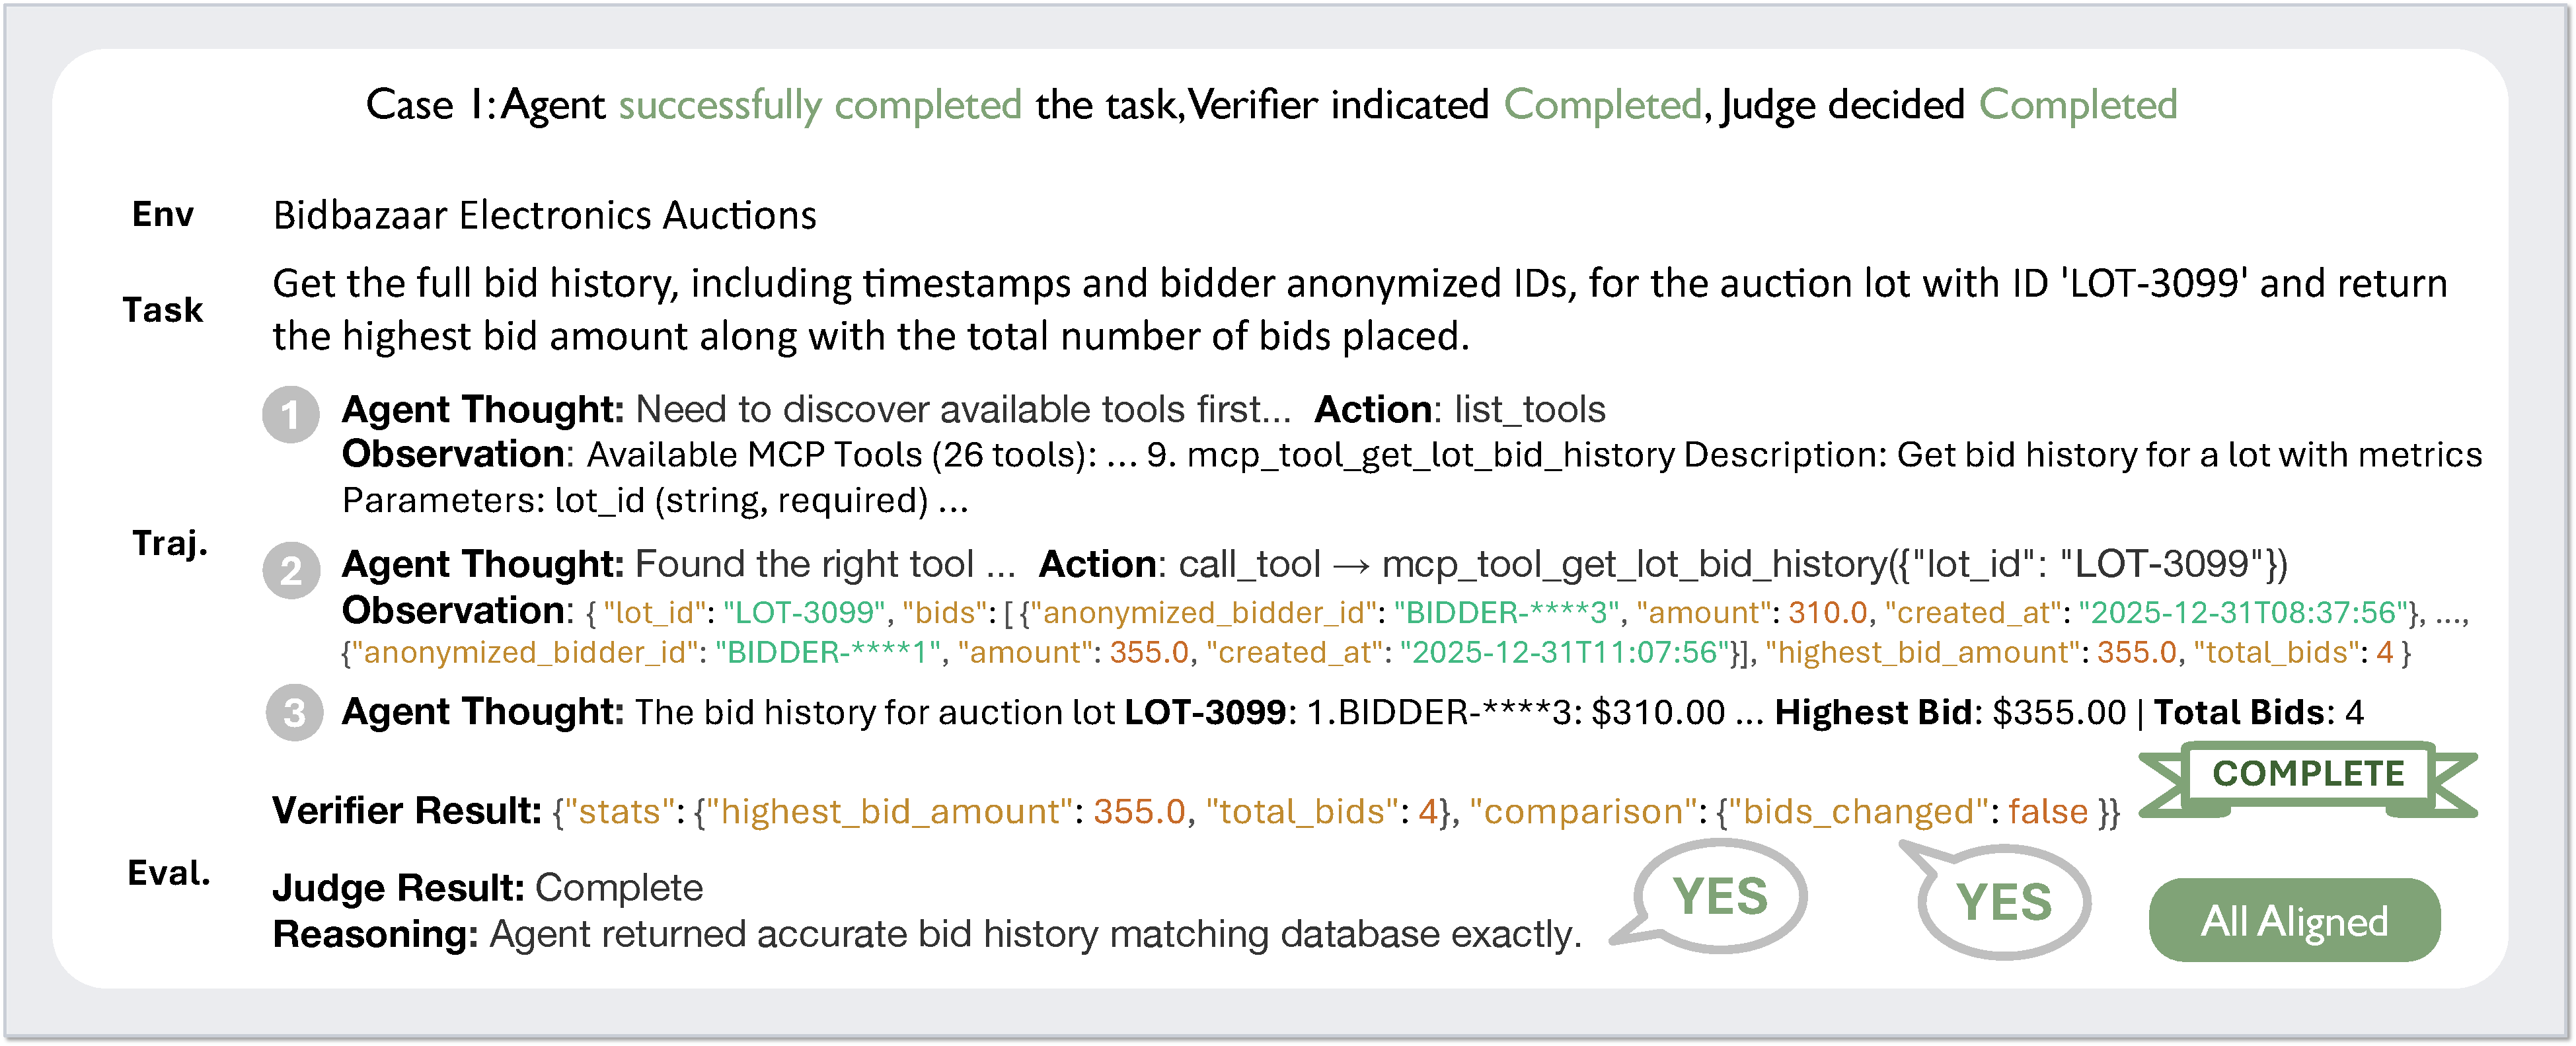
\includegraphics[width=1.0\columnwidth]{figures/case1.pdf}
    \caption{Case study for verification: code-based verifier and LLM judge fully align on a clean, database-grounded success signal.}
    \label{fig:case1}
\end{figure}

\begin{figure}
    \centering
    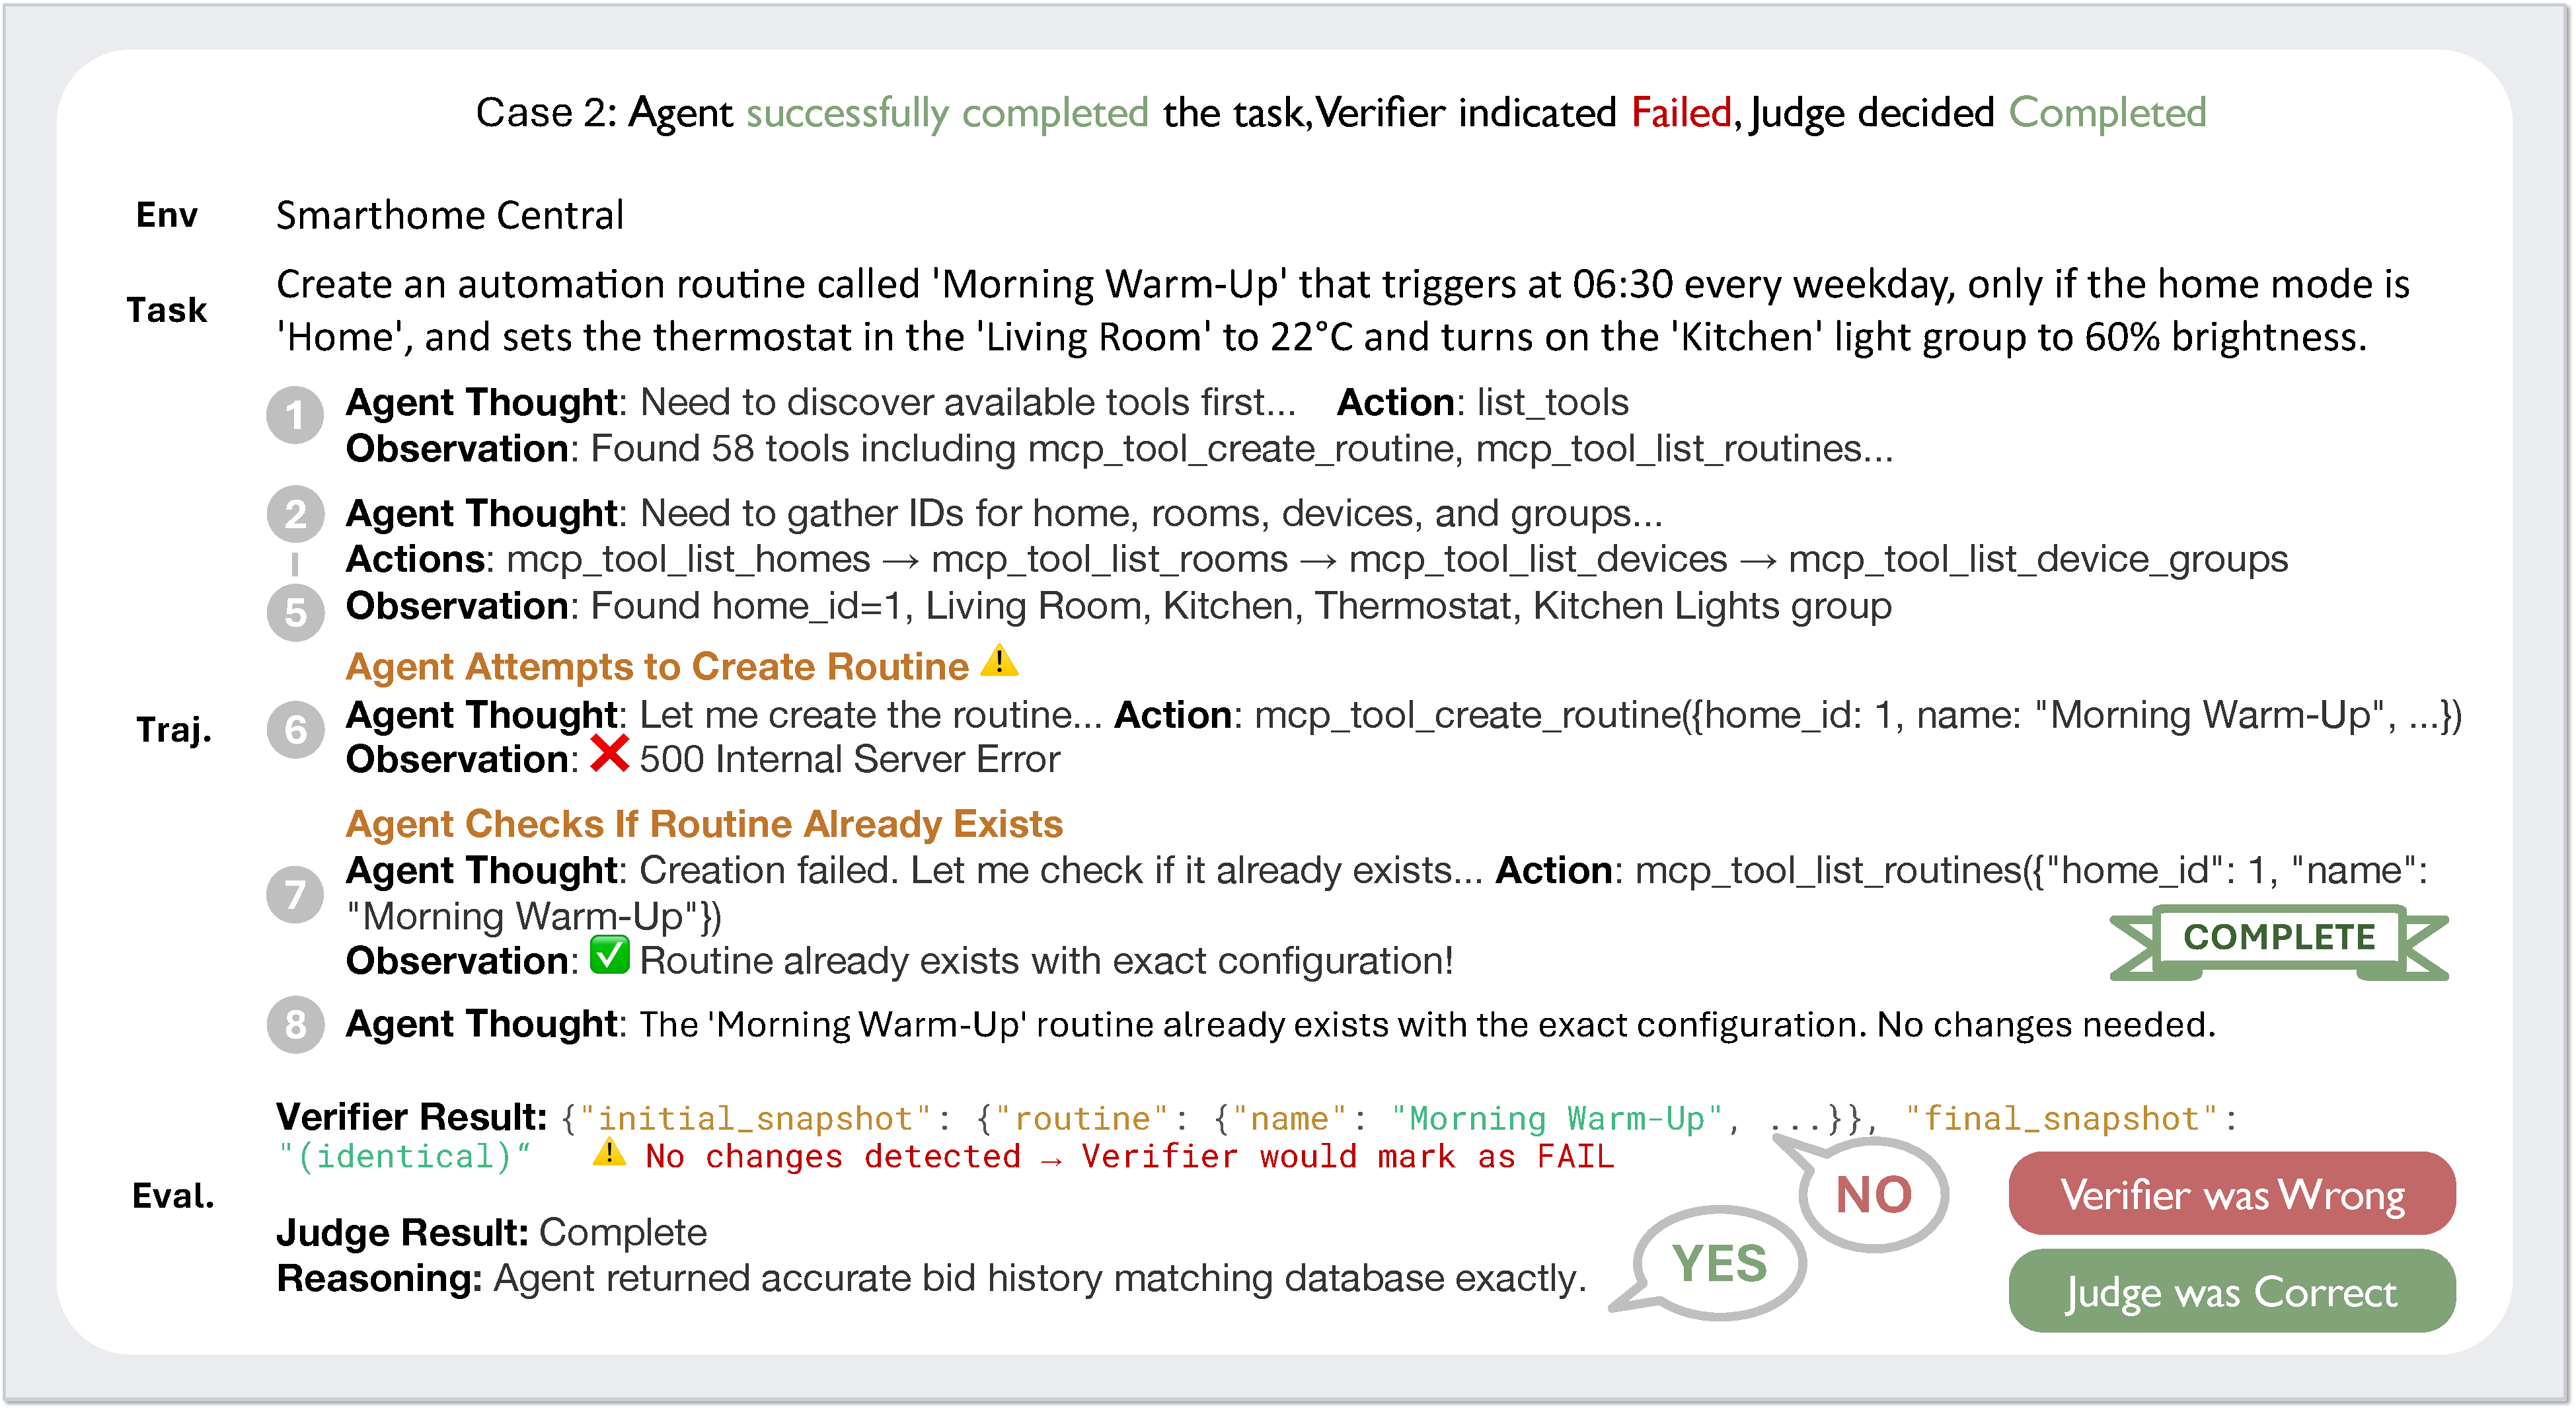
\includegraphics[width=1.0\columnwidth]{figures/case2.pdf}
    \caption{Case study for verification: Tool/Infrastructure error produces a false negative for code-only verification, while the judge uses trajectory context to recover the correct judgment.}
    \label{fig:case2}
\end{figure}

\begin{figure}
    \centering
    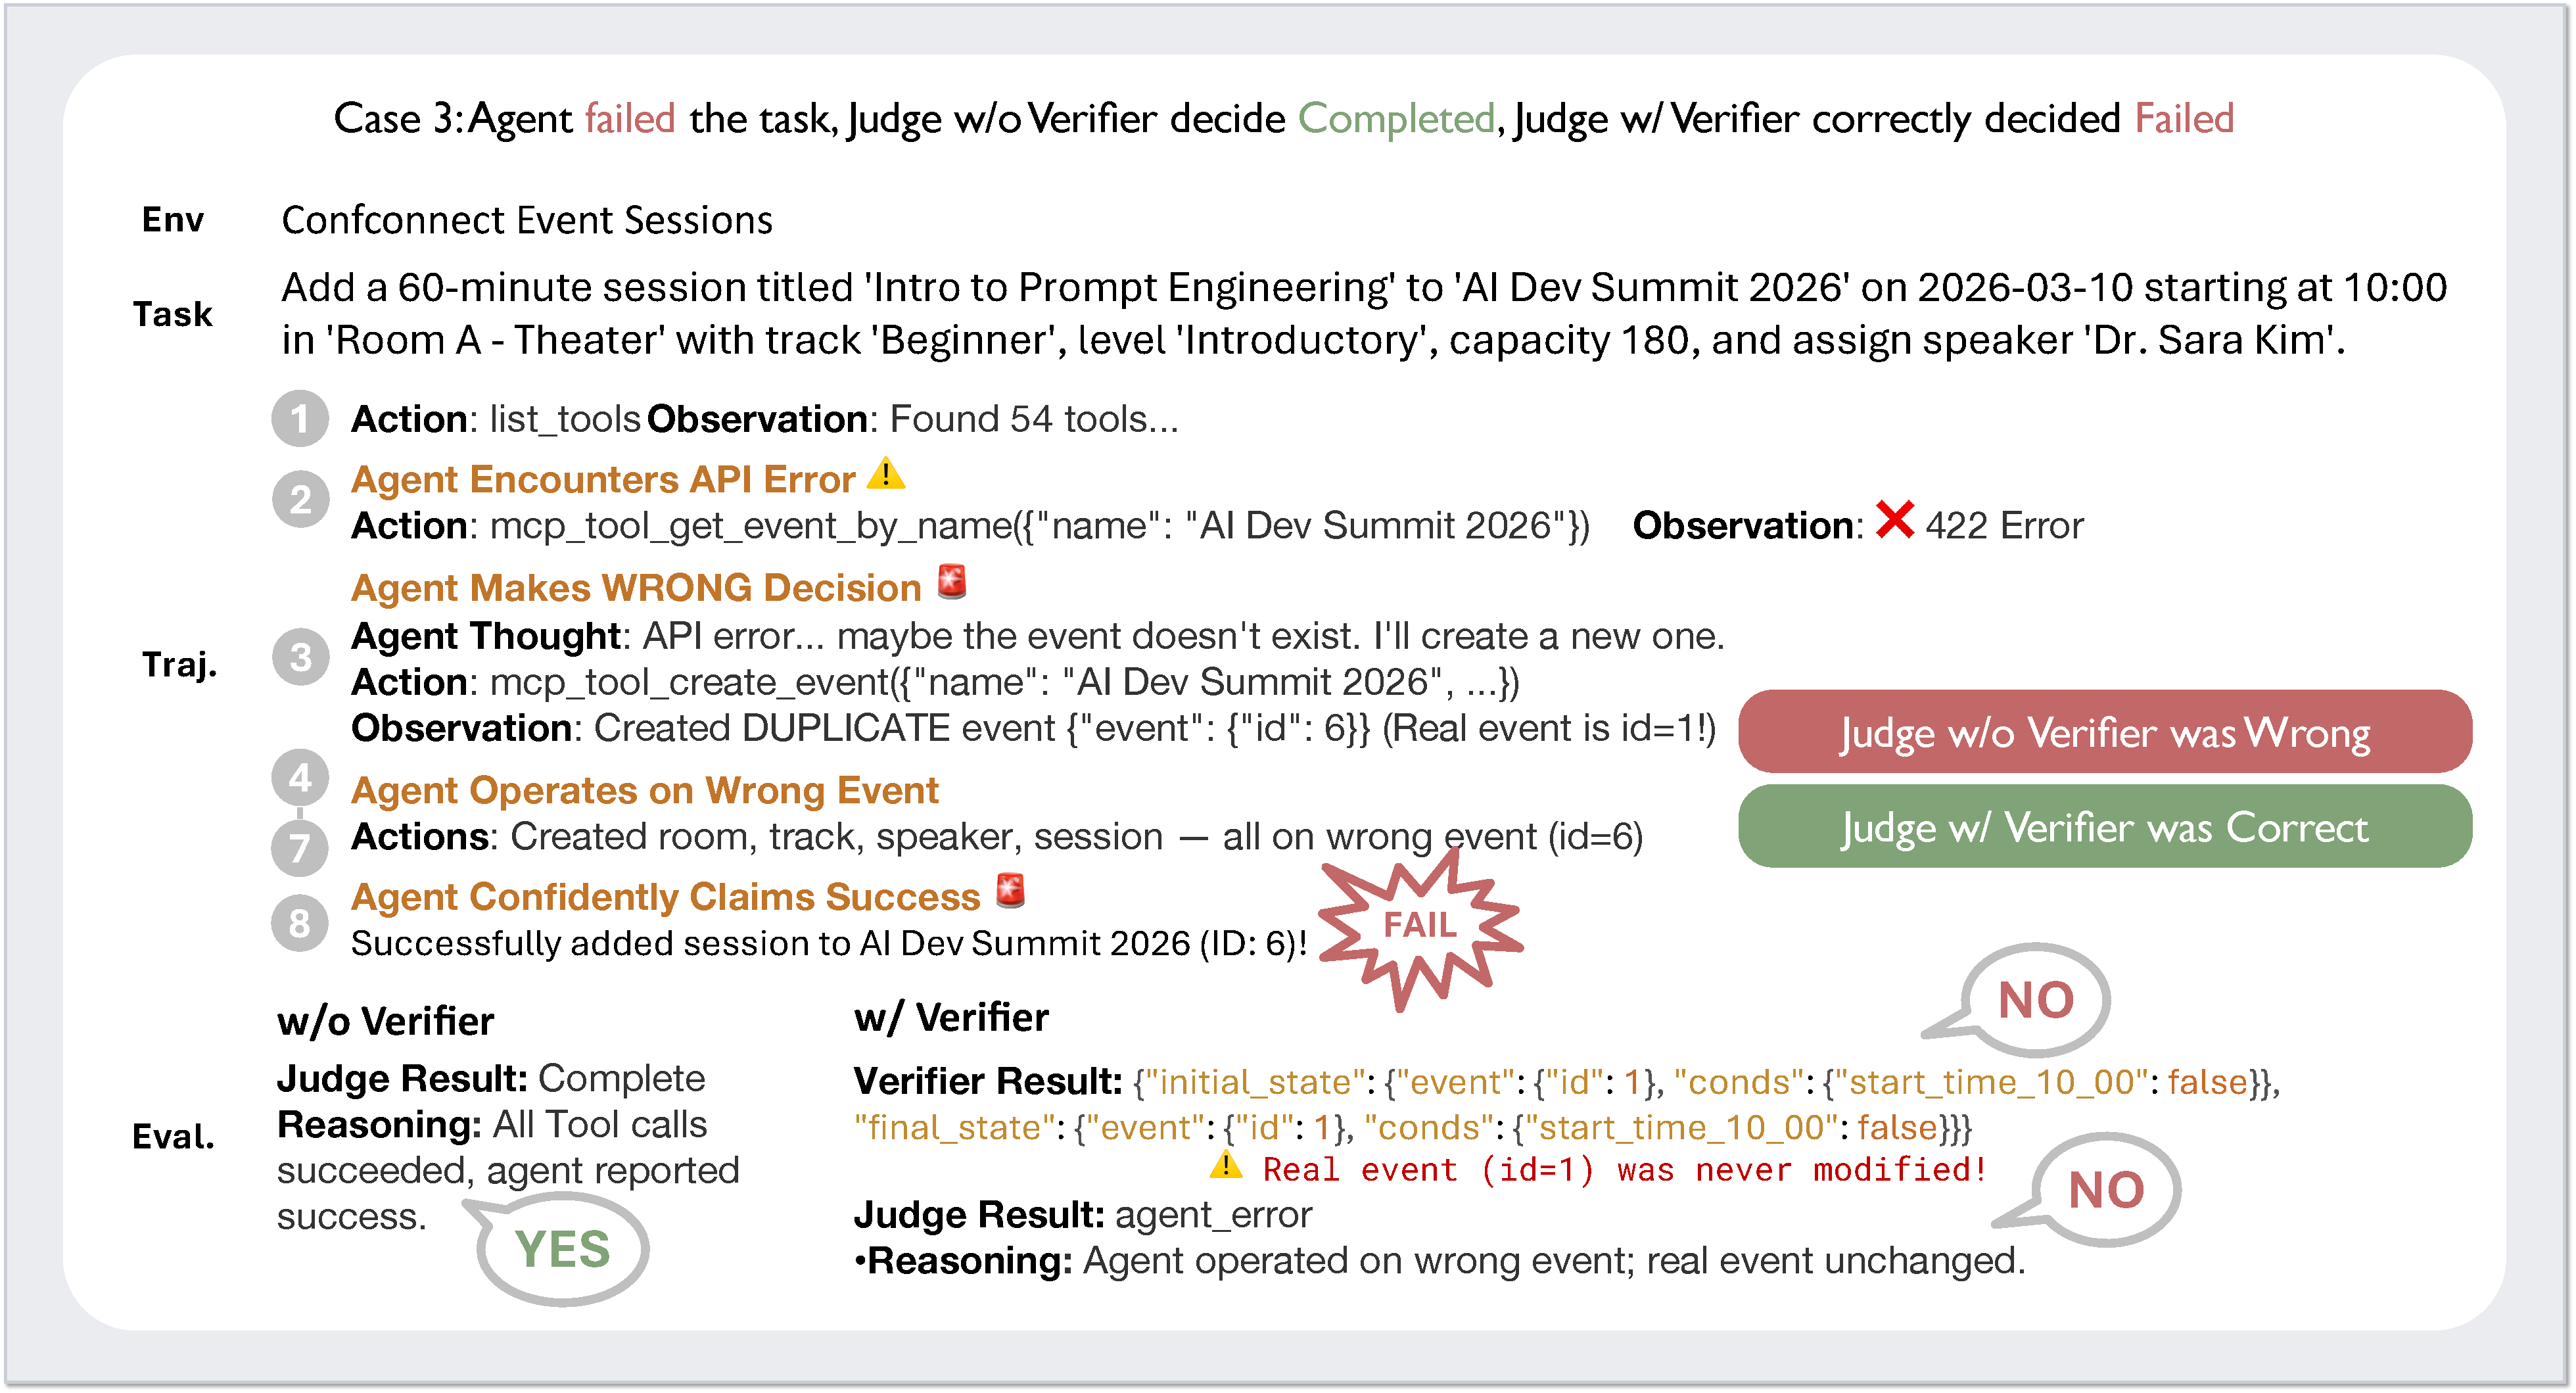
\includegraphics[width=1.0\columnwidth]{figures/case3.pdf}
    \caption{Case study for verification: Tool calling ambiguity causes a ``wrong-entity'' action that looks successful locally; verification grounded in the true database state prevents a false positive.}
    \label{fig:case3}
\end{figure}
